
\documentclass{article}

\usepackage{microtype}
\usepackage{graphicx}
\usepackage{subfigure}
\usepackage{booktabs} %


\usepackage{hyperref}

\newcommand{\theHalgorithm}{\arabic{algorithm}}

\usepackage[preprint]{icml2025}


\usepackage{amsmath}
\usepackage{amssymb}
\usepackage{mathtools}
\usepackage{amsthm}

\usepackage[capitalize, noabbrev]{cleveref}

\theoremstyle{plain}
\newtheorem{theorem}{Theorem}[section]
\newtheorem{proposition}[theorem]{Proposition}
\newtheorem{lemma}[theorem]{Lemma}
\newtheorem{corollary}[theorem]{Corollary}
\theoremstyle{definition}
\newtheorem{definition}[theorem]{Definition}
\newtheorem{assumption}[theorem]{Assumption}
\theoremstyle{remark}
\newtheorem{remark}[theorem]{Remark}

\usepackage[textsize=tiny]{todonotes}

\usepackage{multirow}
%%%%% NEW MATH DEFINITIONS %%%%%

% \usepackage{amsmath,amsfonts,bm}
\usepackage{amsmath,amsfonts}

\usepackage{pifont}


\newcommand{\R}{\mathbb{R}}


\def\va{{\mathbf{a}}}
\def\vg{{\mathbf{g}}}

% Sets
\def\sR{\mathbb{R}}
\def\sC{\mathbb{C}}
\def\sZ{\mathbb{Z}}
\def\sN{\mathbb{N}}
\def\sQ{\mathbb{Q}}

\def\sS{\mathcal{S}}



% Vectors
\def\vzero{{\mathbf{0}}}
\def\vone{{\mathbf{1}}}
\def\vmu{{\mathbf{\mu}}}
\def\vtheta{{\mathbf{\theta}}}
\def\va{{\mathbf{a}}}
\def\vb{{\mathbf{b}}}
\def\vc{{\mathbf{c}}}
\def\vd{{\mathbf{d}}}
\def\ve{{\mathbf{e}}}
\def\vf{{\mathbf{f}}}
\def\vg{{\mathbf{g}}}
\def\vh{{\mathbf{h}}}
\def\vi{{\mathbf{i}}}
\def\vj{{\mathbf{j}}}
\def\vk{{\mathbf{k}}}
\def\vl{{\mathbf{l}}}
\def\vm{{\mathbf{m}}}
\def\vn{{\mathbf{n}}}
\def\vo{{\mathbf{o}}}
\def\vp{{\mathbf{p}}}
\def\vq{{\mathbf{q}}}
\def\vr{{\mathbf{r}}}
\def\vs{{\mathbf{s}}}
\def\vt{{\mathbf{t}}}
\def\vu{{\mathbf{u}}}
\def\vv{{\mathbf{v}}}
\def\vw{{\mathbf{w}}}
\def\vx{{\mathbf{x}}}
\def\vy{{\mathbf{y}}}
\def\vz{{\mathbf{z}}}
\def\vzeta{{\mathbf{\zeta}}}

% Matrix
\def\mA{{\mathbf{A}}}
\def\mB{{\mathbf{B}}}
\def\mC{{\mathbf{C}}}
\def\mD{{\mathbf{D}}}
\def\mE{{\mathbf{E}}}
\def\mF{{\mathbf{F}}}
\def\mG{{\mathbf{G}}}
\def\mH{{\mathbf{H}}}
\def\mI{{\mathbf{I}}}
\def\mJ{{\mathbf{J}}}
\def\mK{{\mathbf{K}}}
\def\mL{{\mathbf{L}}}
\def\mM{{\mathbf{M}}}
\def\mN{{\mathbf{N}}}
\def\mO{{\mathbf{O}}}
\def\mP{{\mathbf{P}}}
\def\mQ{{\mathbf{Q}}}
\def\mR{{\mathbf{R}}}
\def\mS{{\mathbf{S}}}
\def\mT{{\mathbf{T}}}
\def\mU{{\mathbf{U}}}
\def\mV{{\mathbf{V}}}
\def\mW{{\mathbf{W}}}
\def\mX{{\mathbf{X}}}
\def\mY{{\mathbf{Y}}}
\def\mZ{{\mathbf{Z}}}
\def\mBeta{{\mathbf{\beta}}}
\def\mPhi{{\mathbf{\Phi}}}
\def\mLambda{{\mathbf{\Lambda}}}
\def\mSigma{{\mathbf{\Sigma}}}


% Expectation
% \def\eE{\mathop{\mathbb{E}}\limits}
\def\eE{\mathbb{E}}

% Probability
\def\pP{\mathbb{P}}

% Tilde
\def\tf{\tilde{f}}
\def\tS{\tilde{S}}
\def\wtF{\widetilde{\mathcal{F}}}
\def\whR{\widehat{R}}
\def\tvx{\tilde{\mathbf{x}}}
\def\ty{\tilde{y}}


\def\defeq{\overset{\textup{def}}{=}}
% \def\defeq{\overset{.}{=}}
\def\defone{\overset{\text{\ding{172}}}{=}}
\def\deftwo{\overset{\text{\ding{173}}}{=}}
\def\leqone{\overset{\text{\ding{172}}}{\leq}}
\def\leqtwo{\overset{\text{\ding{173}}}{\leq}}
\def\leqthree{\overset{\text{\ding{174}}}{\leq}}
\def\leqfour{\overset{\text{\ding{175}}}{\leq}}
\def\eqone{\overset{\text{\ding{172}}}{=}}
\def\eqtwo{\overset{\text{\ding{173}}}{=}}
\def\eqthree{\overset{\text{\ding{174}}}{=}}
\def\eqfour{\overset{\text{\ding{175}}}{=}}
\def\geqfive{\overset{\text{\ding{176}}}{\geq}}
\definecolor{lightgray}{gray}{.95}
\definecolor{lightyellow}{rgb}{1.0, 1.0, 0.88}
\definecolor{whitesmoke}{rgb}{0.96, 0.96, 0.96}
\definecolor{lightcyan}{rgb}{0.88, 1.0, 1.0}
\usepackage{thmtools}
\newcommand{\jiazheng}[1]{\textcolor{red}{[Jiazheng: #1]}}
\usepackage{siunitx}
\usepackage{titletoc}

\usepackage{hyperref}
\definecolor{cvprblue}{rgb}{0.21,0.49,0.74}
\definecolor{citecolor}{HTML}{2980b9}
\definecolor{linkcolor}{HTML}{c0392b}
\hypersetup{
    colorlinks=true,
    linkcolor=linkcolor,
    citecolor=citecolor,     
    urlcolor=linkcolor,
}

\usepackage{lipsum}
\usepackage{tikz}
\usepackage{multicol}
\usepackage{pifont}

\usepackage[ruled,vlined]{algorithm2e}
\SetKw{KwInit}{Init:}
\usepackage{tcolorbox}
\tcbuselibrary{breakable}

\newtcolorbox{introbox}{colback=gray!10!white, colframe=gray!50!black, boxrule=0.5pt, arc=2pt, left=2pt, right=2pt, top=2pt, bottom=2pt, breakable, width=\linewidth}
\newtcolorbox{initbox}{colback=yellow!10!white, colframe=yellow!50!black, boxrule=0.5pt, arc=2pt, left=2pt, right=2pt, top=2pt, bottom=2pt, breakable, width=\linewidth}
\newtcolorbox{optbox}{colback=blue!10!white, colframe=blue!50!black, boxrule=0.5pt, arc=2pt, left=2pt, right=2pt, top=2pt, bottom=2pt, breakable, width=0.933\linewidth}
\newtcolorbox{updatebox}{colback=green!10!white, colframe=green!50!black, boxrule=0.5pt, arc=2pt, left=2pt, right=2pt, top=2pt, bottom=2pt, breakable, width=0.866\linewidth}

\usepackage{enumitem}




\begin{document}
    \twocolumn[ \icmltitle{Scalable Model Merging with Progressive Layer-wise Distillation}




    \begin{icmlauthorlist}
        \icmlauthor{Jing Xu}{thu} 
        \icmlauthor{Jiazheng Li}{bit}
        \icmlauthor{Jingzhao Zhang}{thu,sqz}
    \end{icmlauthorlist}

    \icmlaffiliation{thu}{Institute for Interdisciplinary Information Sciences, Tsinghua University}
    \icmlaffiliation{bit}{School of Computer Science, Beijing Institute of Technology} 
    \icmlaffiliation{sqz}{Shanghai Qizhi Institute}

    \icmlcorrespondingauthor{Jing Xu}{xujing21@mails.tsinghua.edu.cn} 

    \icmlkeywords{Machine Learning, ICML}

    \vskip 0.3in ]



    \printAffiliationsAndNotice{}

    

    \begin{abstract}
Retrieval-Augmented Generation (RAG) is often used with Large Language Models (LLMs) to infuse domain knowledge or user-specific information. In RAG, given a user query, a retriever extracts chunks of relevant text from a knowledge base. These chunks are sent to an LLM as part of the input prompt. Typically, any given chunk is repeatedly retrieved across user questions. However, currently, for every question, attention-layers in LLMs fully compute the key values (KVs) repeatedly for the input chunks, as state-of-the-art methods cannot reuse KV-caches when chunks appear at arbitrary locations with arbitrary contexts. Naive reuse leads to output quality degradation.  This leads to potentially redundant computations on expensive GPUs and increases latency. In this work, we propose \sys, a system for managing and reusing precomputed KVs corresponding to the text chunks (we call \textit{chunk-caches}) in RAG-based systems. We present how to identify \hl{\textit{chunk-caches} that are reusable}, how to efficiently perform a small fraction of recomputation to \textit{fix} the cache to maintain output quality, and how to efficiently store and evict \textit{chunk-caches} in the hardware for maximizing reuse while masking any overheads. With real production workloads as well as synthetic datasets, we show that \sys reduces redundant computation by \textbf{51\%} over SOTA prefix-caching and \textbf{75\%} over full recomputation.
\hl{Additionally, with continuous batching on a real production workload, we get a \textbf{1.6$\times$} speedup in throughput and a \textbf{2$\times$} reduction in end-to-end response latency over prefix-caching while maintaining quality, for both the \llama-3-8B and \llama-3-70B models. 
}
\end{abstract}





    \section{Introduction}
\label{sec:intro}

\begin{figure*}[tb]
    \centering
    \includegraphics[width=0.848\linewidth]{figs/circuitnn.pdf} 
    \caption{Illustration of differentiable CircuitNN. CircuitNN is designed based on differentiable NAND gates. After DAS is guided by PI and PO pairs of the truth table, CircuitNN can get the precise circuit architecture logic equivalent to the truth table.}
    \label{fig:circuitnn}
\end{figure*}

% 1. Describe the importance of logic synthesis
% 2. Existing Problems
% (a) Neural Architecture Search: Unstable, Predefined Setting, etc.
% (b) Circuit Generation: Probabilistic Model, Logic Equivalence

With the rapid advancement of technology, the scale of integrated circuits (ICs) has expanded exponentially. 
This expansion has introduced significant challenges in chip manufacturing, particularly concerning power and area metrics.
A primary objective in IC design is achieving the same circuit function with fewer transistors, thereby reducing power usage and area occupancy.

Logic synthesis~\cite{hachtel2005logicsynth}, a critical step in electronic design automation (EDA), transforms behavioral-level circuit designs into optimized gate-level circuits, ultimately yielding the final IC layout. 
The primary goal of logic synthesis is to identify the physical implementation with the fewest gates for a given circuit function. 
This task constitutes a challenging NP-hard combinatorial optimization problem. 
Current logic synthesis tools~\cite{brayton2010abc, wolf2013yosys} rely on human-designed heuristics, often leading to sub-optimal outcomes.

Differentiable architecture search (DAS) techniques~\cite{liu2018darts, chu2020darts} offer novel perspectives on addressing challenges in this problem.
Circuit functions can be represented through truth tables, which map binary inputs to their corresponding outputs. 
Truth tables provide a precise representation of input-output relationships, ensuring the design of functionally equivalent circuits.
Inspired by this, researchers~\cite{deepmind2024ai4sys, wang2024tnet} have begun exploring the application of DAS to synthesize circuits directly from truth tables.
Specifically, \citet{deepmind2024ai4sys} proposed CircuitNN, a framework that learns differentiable connection structures with logic gates, enabling the automatic generation of logic circuits from truth tables.
This approach significantly reduces the complexity of traditional circuit generation. 
Building on this, \citet{wang2024tnet} introduced T-Net, a triangle-shaped variant of CircuitNN, incorporating regularization techniques to enhance the efficiency of DAS.

Despite these advancements, several challenges remain. 
The computational complexity of DAS grows quadratically with the number of gates, posing scalability issues.
Although triangle-shaped architecture~\cite{wang2024tnet} partially mitigates this problem, redundancy persists. 
%Additionally, DAS is susceptible to converging to local optima, limiting the ability to search architectures that satisfy the given truth tables~\cite{liu2018darts}. 
%Furthermore, hyperparameters (network depth and layer width) require extensive searches, introducing complexity and prolonging the synthesis process. 
Additionally, DAS is susceptible to converging to local optima~\cite{liu2018darts} and hyperparameters (network depth and layer width) require extensive searches. 
The challenges arise from the vast search space in DAS. 
% Even with predefined settings for CircuitNN, finding a configuration that meets the truth table requires extensive trial and error during the DAS process. 
Intuitively, limiting the search space through predefined parameters (network depth, gates per layer, and connection probabilities) can significantly reduce the complexity.

Recent advances~\cite{openai2023gpt4, abramson2024alphafold3, esser2024sd3, li2024mar} in conditional generative models have demonstrated remarkable performance across language, vision, and graph generation tasks. 
Motivated by these developments, we propose a novel approach to circuit generation that generates preliminary circuit structures to guide DAS in generating refined circuits matching specified truth tables. 
Firstly, we introduce CircuitVQ, a tokenizer with a discrete codebook for circuit tokenization. 
Built upon our Circuit AutoEncoder framework~\cite{hou2022graphmae,li2023maskgae,wu2025mgvga}, CircuitVQ is trained through a circuit reconstruction task. 
Specifically, the CircuitVQ encoder encodes input circuits into discrete tokens using a learnable codebook, while the decoder reconstructs the circuit adjacency matrix based on these tokens.
Subsequently, the CircuitVQ encoder serves as a circuit tokenizer for CircuitAR pretraining, which employs a masked autoregressive modeling paradigm~\cite{chang2022maskgit, li2023mage}. 
In this process, the discrete codes function as supervision signals. 
After training, CircuitAR can generate discrete tokens progressively, which can be decoded into initial circuit structures by the decoder of the CircuitVQ. 
These prior insights can guide DAS in producing refined circuits that match the target truth tables precisely.

Our key contributions can be summarized as follows:
\begin{itemize}
\item We introduce CircuitVQ, a circuit tokenizer that facilitates graph autoregressive modeling for circuit generation, based on our Circuit AutoEncoder framework;
\item Develop CircuitAR, a model trained using masked autoregressive modeling, which generates initial circuit structures conditioned on given truth tables;
\item Propose a refinement framework that integrates differentiable architecture search to produce functionally equivalent circuits guided by target truth tables;
\item Comprehensive experiments demonstrating the scalability and capability emergence of our CircuitAR and the superior performance of the proposed circuit generation approach.
\end{itemize}

% Motivation
% (a) Diffusion (Vision, Graph), Autoregressive (Language, Vision)
% (b) Circuit Generation for Predefined Setting
% (c) Neural Architecture Search for Strict Logic Equivalence

% Contribution
% (a) Circuit Tokenizer (new transformer arch, training strategy)
% (b) CircuitAR (train and gen strategies, post-ar strategy)
% (c) Extensive Evaluation including BitD (Bit Distance) for Scalability

    \section{Preliminary}

\paragraph{Notation} Consider a sentence of $T$ tokens $\vx=\{\vx_1,\ldots, \vx_T\}\in\gX$, and let $P$ be the unknown target language distribution, $\tilde P(\vx)$ be the empirical distribution of the training data (which is an approximation of $P$), and $Q$ be the distribution of our model at hand. Since our paper is also closely related to RLHF, we will also use $\pi$ to represent the distributions. In particular, we sometimes write $\pi_\theta$ for a distribution that is parameterized by $\theta$, where $\theta$ is usually the set of trainable parameters of the LLM; we write $\pr$ for a reference distribution that should be clear given the context. The next token prediction loss is minimizing the forward-KL between $P$ and $Q$. 




    \section{Experiments}
\label{sec:Experiments} 

We conduct several experiments across different problem settings to assess the efficiency of our proposed method. Detailed descriptions of the experimental settings are provided in \cref{sec:apendix_experiments}.
%We conduct experiments on optimizing PINNs for convection, wave PDEs, and a reaction ODE. 
%These equations have been studied in previous works investigating difficulties in training PINNs; we use the formulations in \citet{krishnapriyan2021characterizing, wang2022when} for our experiments. 
%The coefficient settings we use for these equations are considered challenging in the literature \cite{krishnapriyan2021characterizing, wang2022when}.
%\cref{sec:problem_setup_additional} contains additional details.

%We compare the performance of Adam, \lbfgs{}, and \al{} on training PINNs for all three classes of PDEs. 
%For Adam, we tune the learning rate by a grid search on $\{10^{-5}, 10^{-4}, 10^{-3}, 10^{-2}, 10^{-1}\}$.
%For \lbfgs, we use the default learning rate $1.0$, memory size $100$, and strong Wolfe line search.
%For \al, we tune the learning rate for Adam as before, and also vary the switch from Adam to \lbfgs{} (after 1000, 11000, 31000 iterations).
%These correspond to \al{} (1k), \al{} (11k), and \al{} (31k) in our figures.
%All three methods are run for a total of 41000 iterations.

%We use multilayer perceptrons (MLPs) with tanh activations and three hidden layers. These MLPs have widths 50, 100, 200, or 400.
%We initialize these networks with the Xavier normal initialization \cite{glorot2010understanding} and all biases equal to zero.
%Each combination of PDE, optimizer, and MLP architecture is run with 5 random seeds.

%We use 10000 residual points randomly sampled from a $255 \times 100$ grid on the interior of the problem domain. 
%We use 257 equally spaced points for the initial conditions and 101 equally spaced points for each boundary condition.

%We assess the discrepancy between the PINN solution and the ground truth using $\ell_2$ relative error (L2RE), a standard metric in the PINN literature. Let $y = (y_i)_{i = 1}^n$ be the PINN prediction and $y' = (y'_i)_{i = 1}^n$ the ground truth. Define
%\begin{align*}
%    \mathrm{L2RE} = \sqrt{\frac{\sum_{i = 1}^n (y_i - y'_i)^2}{\sum_{i = 1}^n y'^2_i}} = \sqrt{\frac{\|y - y'\|_2^2}{\|y'\|_2^2}}.
%\end{align*}
%We compute the L2RE using all points in the $255 \times 100$ grid on the interior of the problem domain, along with the 257 and 101 points used for the initial and boundary conditions.

%We develop our experiments in PyTorch 2.0.0 \cite{paszke2019pytorch} with Python 3.10.12.
%Each experiment is run on a single NVIDIA Titan V GPU using CUDA 11.8.
%The code for our experiments is available at \href{https://github.com/pratikrathore8/opt_for_pinns}{https://github.com/pratikrathore8/opt\_for\_pinns}.


\subsection{2D Allen Cahn Equation}
\begin{figure*}[t]
    \centering
    \includegraphics[scale=0.38]{figs/Burgers_operator.pdf}
    \caption{1D Burgers' Equation (Operator Learning): Steady-state solutions for different initializations $u_0$ under varying viscosity $\varepsilon$: (a) $\varepsilon = 0.5$, (b) $\varepsilon = 0.1$, (c) $\varepsilon = 0.05$. The results demonstrate that all final test solutions converge to the correct steady-state solution. (d) Illustration of the evolution of a test initialization $u_0$ following homotopy dynamics. The number of residual points is $\nres = 128$.}
    \label{fig:Burgers_result}
\end{figure*}
First, we consider the following time-dependent problem:
\begin{align}
& u_t = \varepsilon^2 \Delta u - u(u^2 - 1), \quad (x, y) \in [-1, 1] \times [-1, 1] \nonumber \\
& u(x, y, 0) = - \sin(\pi x) \sin(\pi y) \label{eq.hom_2D_AC}\\
& u(-1, y, t) = u(1, y, t) = u(x, -1, t) = u(x, 1, t) = 0. \nonumber
\end{align}
We aim to find the steady-state solution for this equation with $\varepsilon = 0.05$ and define the homotopy as:
\begin{equation}
    H(u, s, \varepsilon) = (1 - s)\left(\varepsilon(s)^2 \Delta u - u(u^2 - 1)\right) + s(u - u_0),\nonumber
\end{equation}
where $s \in [0, 1]$. Specifically, when $s = 1$, the initial condition $u_0$ is automatically satisfied, and when $s = 0$, it recovers the steady-state problem. The function $\varepsilon(s)$ is given by
\begin{equation}
\varepsilon(s) = 
\left\{\begin{array}{l}
s, \quad s \in [0.05, 1], \\
0.05, \quad s \in [0, 0.05].
\end{array}\right.\label{eq:epsilon_t}
\end{equation}

Here, $\varepsilon(s)$ varies with $s$ during the first half of the evolution. Once $\varepsilon(s)$ reaches $0.05$, it remains fixed, and only $s$ continues to evolve toward $0$. As shown in \cref{fig:2D_Allen_Cahn_Equation}, the relative $L_2$ error by homotopy dynamics is $8.78 \times 10^{-3}$, compared with the result obtained by PINN, which has a $L_2$ error of $9.56 \times 10^{-1}$. This clearly demonstrates that the homotopy dynamics-based approach significantly improves accuracy.

\subsection{High Frequency Function Approximation }
We aim to approximate the following function:
$u=    \sin(50\pi x), \quad x \in [0,1].$
The homotopy is defined as $H(u,\varepsilon) = u - \sin(\frac{1}{\varepsilon}\pi x), $
where $\varepsilon \in [\frac{1}{50},\frac{1}{15}]$.

\begin{table}[htbp!]
    \caption{Comparison of the lowest loss achieved by the classical training and homotopy dynamics for different values of $\varepsilon$ in approximating $\sin\left(\frac{1}{\varepsilon} \pi x\right)$
    }
    \vskip 0.15in
    \centering
    \tiny
    \begin{tabular}{|c|c|c|c|c|} 
    \hline 
    $ $ & $\varepsilon = 1/15$ & $\varepsilon = 1/35$ & $\varepsilon = 1/50$ \\ \hline 
    Classical Loss                & 4.91e-6     & 7.21e-2     & 3.29e-1       \\ \hline 
    Homotopy Loss $L_H$                      & 1.73e-6     & 1.91e-6     & \textbf{2.82e-5}       \\ \hline
    \end{tabular}
    % On convection, \al{} provides 14.2$\times$ and 1.97$\times$ improvement over Adam or \lbfgs{} on L2RE. 
    % On reaction, \al{} provides 1.10$\times$ and 1.99$\times$ improvement over Adam or \lbfgs{} on L2RE.
    % On wave, \al{} provides 6.32$\times$ and 6.07$\times$ improvement over Adam or \lbfgs{} on L2RE.}
    \label{tab:loss_approximate}
\end{table}

As shown in \cref{fig:high_frequency_result}, due to the F-principle \cite{xu2024overview}, training is particularly challenging when approximating high-frequency functions like $\sin(50\pi x)$. The loss decreases slowly, resulting in poor approximation performance. However, training based on homotopy dynamics significantly reduces the loss, leading to a better approximation of high-frequency functions. This demonstrates that homotopy dynamics-based training can effectively facilitate convergence when approximating high-frequency data. Additionally, we compare the loss for approximating functions with different frequencies $1/\varepsilon$ using both methods. The results, presented in \cref{tab:loss_approximate}, show that the homotopy dynamics training method consistently performs well for high-frequency functions.





\subsection{Burgers Equation}
In this example, we adopt the operator learning framework to solve for the steady-state solution of the Burgers equation, given by:
\begin{align}
& u_t+\left(\frac{u^2}{2}\right)_x - \varepsilon u_{xx}=\pi \sin (\pi x) \cos (\pi x), \quad x \in[0, 1]\nonumber\\
& u(x, 0)=u_0(x),\label{eq:1D_Burgers} \\
& u(0, t)=u(1, t)=0, \nonumber 
\end{align}
with Dirichlet boundary conditions, where $u_0 \in L_{0}^2((0, 1); \mathbb{R})$ is the initial condition and $\varepsilon \in \mathbb{R}$ is the viscosity coefficient. We aim to learn the operator mapping the initial condition to the steady-state solution, $G^{\dagger}: L_{0}^2((0, 1); \mathbb{R}) \rightarrow H_{0}^r((0, 1); \mathbb{R})$, defined by $u_0 \mapsto u_{\infty}$ for any $r > 0$. As shown in Theorem 2.2 of \cite{KREISS1986161} and Theorems 2.5 and 2.7 of \cite{hao2019convergence}, for any $\varepsilon > 0$, the steady-state solution is independent of the initial condition, with a single shock occurring at $x_s = 0.5$. Here, we use DeepONet~\cite{lu2021deeponet} as the network architecture. 
The homotopy definition, similar to ~\cref{eq.hom_2D_AC}, can be found in \cref{Ap:operator}. The results can be found in \cref{fig:Burgers_result} and \cref{tab:loss_burgers}. Experimental results show that the homotopy dynamics strategy performs well in the operator learning setting as well.


\begin{table}[htbp!]
    \caption{Comparison of loss between classical training and homotopy dynamics for different values of $\varepsilon$ in the Burgers equation, along with the MSE distance to the ground truth shock location, $x_s$.}
    \vskip 0.15in
    \centering
    \tiny
    \begin{tabular}{|c|c|c|c|c|} 
    \hline  
    $ $ & $\varepsilon = 0.5$ & $\varepsilon = 0.1$ & $\varepsilon = 0.05$ \\ \hline 
    Homotopy Loss $L_H$                &  7.55e-7     & 3.40e-7     & 7.77e-7       \\ \hline 
    L2RE                      & 1.50e-3     & 7.00e-4     & 2.52e-2       \\ \hline
        MSE Distance $x_s$                      & 1.75e-8     & 9.14e-8      & 1.2e-3      \\ \hline
    \end{tabular}
    % On convection, \al{} provides 14.2$\times$ and 1.97$\times$ improvement over Adam or \lbfgs{} on L2RE. 
    % On reaction, \al{} provides 1.10$\times$ and 1.99$\times$ improvement over Adam or \lbfgs{} on L2RE.
    % On wave, \al{} provides 6.32$\times$ and 6.07$\times$ improvement over Adam or \lbfgs{} on L2RE.}
    \label{tab:loss_burgers}
\end{table}



% \begin{itemize}
%     \item Relate the curvature in the problem to the differential operator. Use this to demonstrate why the problem is ill-conditioned
%     \item Give an argument for why using Adam + L-BFGS is better than just using L-BFGS outright. The idea is that Adam lowers the errors to the point where the rest of the optimization becomes convex \ldots
%     \item Show why we need second-order methods. We would like to prove that once we are close to the optimum, second-order methods will give condition-number free linear convergence. Specialize this to the Gauss-Newton setting, with the randomized low-rank approximation.
%     % \item Show that it is not possible to get superlinear convergence under the interpolation assumption with an overparameterized neural network. This should be true b/c the Hessian at the optimum will have rank $\min(n, d)$, and when $d > n$, this guarantees that we cannot have strong convexity.
% \end{itemize}
    % \begin{figure}
%     \centering
%     \includegraphics[width=0.5\linewidth]{Move_teaser.pdf}
%     \caption{Comparison of different dynamic compute approaches. length of arrow indicates residual transformation per token while width indicates velocity of transformation.}
%     \label{fig:enter-label}
% \end{figure}

\section{Method}
\label{sec:method}
Residual connections play a crucial role in shaping token representations, yet their dynamics remain underexplored in the context of efficient decoding. In this work, we delve deeper into transformer residual dynamics and investigate how modulating residual transformation velocity can improve inference efficiency in token-level processing, optimizing both dense and sparse MoE transformers.


\subsection{Residual Dynamics and Motivation for Multi-rate Residuals} \label{sec:motivation}

To analyze how hidden representations evolve across different layers of a transformer architecture, it's crucial to consider the effect of residual connections. Each transformer decoder layer typically has residual connections across attention and MLP submodules. As the residual stream $h_i$ traverses from interval $E_j$ to $E_{j+1}$, it undergoes a residual transformation given by:  
% \begin{equation}
% \label{eq:slow_residual_transformation}
% H_{E_{j+1}} = H_{E_j} \prod_{i=E_j}^{E_{j+1}} \left( I + \mathcal{A}_i \right) \left( I + \mathcal{M}_i \right) \quad \text{where} \quad \mathcal{A}_i = f(c_i, h_{i}), \mathcal{M}_i = g(h_i)
% \end{equation}

\begin{equation} \label{eq:slow_residual_transformation}
h_{E_{j+1}} = h_{E_j} + \sum_{i=E_j}^{E_{j+1}-1} \left( \mathcal{A}_i(h_i) + \mathcal{M}_i(h_i + \mathcal{A}_i(h_i)) \right) \quad \text{where} \quad \mathcal{A}_i = f(c_i, h_{i}), \mathcal{M}_i = g(h_i). 
\end{equation}

Here, \( \mathcal{A}_i \) denotes the non-linear transformation introduced by the multi-head attention mechanism at layer \( i \), while \( \mathcal{M}_i \) corresponds to the non-linear transformation of the MLP block at the same layer. These transformations depend on the input residual stream \( h_i \) and, in the case of \( \mathcal{A}_i \), the previous contextual representation \( c_i \).\footnote{Normalization layers are typically applied in practice but are omitted here for simplicity of the argument.}


% For easy tokens, the magnitude and direction of this delta transformation become progressively smaller with each successive layer as shown in \cref{fig:delta_transformation}. Consequently, it is feasible to predict these tokens after only a few residual connections, whereas harder tokens necessitate more extensive processing through additional layers.

\begin{figure}[ht]
    \centering
    \begin{subfigure}{0.48\textwidth}
        \centering
        \includegraphics[width=\textwidth]{sections/figures/residual_change.pdf}
        \caption{}
        \label{fig:residual_change}
    \end{subfigure}%
    \hfill
    \begin{subfigure}{0.48\textwidth}
        \centering
        \includegraphics[width=\textwidth]{sections/figures/alignment_wrt_dedicated_model.pdf}
        \caption{}
    \label{fig:alignment_wrt_dedicated_model}
    \end{subfigure}
    \caption{(a) As residual streams propagate through the model, the directional shifts in the residuals become progressively smaller. (b) A dedicated model with $k$ layers achieves a faster rate of change in residual streams and higher alignment than base model leveraging early exit mechanisms at layer $k$.}
    \label{fig}
\end{figure}


To examine whether residual transformations can be accelerated across layers, we conducted experiments using a diverse set of prompts on a pre-trained Phi3 model~\cite{phi3_report}. As illustrated in \cref{fig:residual_change}, we measured the directional shift in residual states as \( 1 - \mathcal{C}(h_{i-1}, h_i) \), where \(\mathcal{C}\) denotes normalized cosine similarity. This shift is notably higher in the initial layers, gradually decreasing in subsequent layers. This behavior allows traditional early exit approaches to effectively accelerate decoding by enabling earlier exits for simpler tokens. However, these approaches typically rely on a distance-based approximation, where the full residual transformation of the model is approximated by the residual transformations of the initial layers. To gain deeper insights into the distance versus velocity aspects of residual transformation, we conducted a comparative study. Specifically, we trained an early exit head at layer $k$ of the Phi3 model, which consists of 32 layers, restricting the distance traveled by each token. To accelerate the residual transformation relative to number of layers, we trained a smaller model consisting of only $k$ layers, while keeping all other hyperparameters consistent. We then compared the next-token prediction accuracy of the early exit head of the base model with that of the smaller model. To ensure an equal number of trainable parameters, we inserted low-rank adapters into the smaller model and trained only these adapters, whereas, in the distance-based approach, we trained solely the early exit head. In addition, to accelerate the residual transformation in smaller model, we distilled the residual streams from the larger model by incorporating a distillation loss ~\cite{sanh2019distilbert} between the residual state at layer \(i\) of the smaller model and the residual state at layer \(4 \times i\) of the larger model. As shown in ~\cref{fig:alignment_wrt_dedicated_model} the smaller model demonstrates a significantly faster rate of change in residual streams, leading to higher next token prediction accuracy after $k$ layers compared to the base model that employs traditional early exit mechanisms after $k$ layers \cite{schuster2022confident, chen2023eellm, varshney-etal-2024-investigating}. This experimental setup, which modifies only the rate of change in residual streams while keeping other factors constant, suggests that dense transformers, trained with a fixed number of layers, may inherently possess a slow residual transformation bias.

This observation raises an intriguing question: if the rate of change in residual streams could be accelerated relative to the number of layers, is it possible to facilitate earlier alignment for a greater proportion of tokens? Earlier alignment would be beneficial to not only facilitate dynamic computation but also for generating speculative tokens efficiently with high acceptance rates in speculative decoding setups ~\cite{leviathan2023fast, chen2023accelerating}. 

%thereby enhancing the efficiency of early exiting? 
 % This bias likely constrains the effectiveness of early exiting, particularly for easier tokens. By addressing this limitation through accelerated residual transformations, we hypothesize that it is possible to substantially improve the efficiency and accuracy of early exit strategies in transformer models.

\subsection{Multi-Rate Residual Transformation} \label{m2r2_method}

To address the slow residual transformation bias described in ~\cref{sec:motivation}, we introduce \textit{accelerated residual streams} that operate at rate $R$ relative to original slow residual stream. We pair slow residual stream, $h$ with an accelerated residual stream, $p$, which has an intrinsic bias towards earlier alignment. Relative to ~\cref{eq:slow_residual_transformation}, accelerated residual transformation from interval $E_j$ to $E_{j+1}$ can be represented as: 

% \begin{equation}
% \label{eq:fast_residual_transformation}
% P_{E_{j+1}} = P_{E_j} \prod_{i=E_j}^{E_{j+1}} \left( I + \hat{\mathcal{A}_i} \right) \left( I + \hat{\mathcal{M}_i} \right) \quad \text{where} \quad \hat{\mathcal{A}_i} = \hat{f}(c_i, P_{i}), \hat{\mathcal{M}_i} = \hat{g}(P_{i})
% \end{equation}


\begin{equation} \label{eq:fast_residual_transformation}
p_{E_{j+1}} = p_{E_j} + \sum_{i=E_j}^{E_{j+1}-1} \left( \hat{\mathcal{A}_i}(p_i) + \hat{\mathcal{M}_i}(p_i + \hat{\mathcal{A}_i}(p_i)) \right) \quad \text{where} \quad \hat{\mathcal{A}_i} = \hat{f}(c_i, p_{i}), \hat{\mathcal{M}_i} = \hat{g}(h_i), 
\end{equation}



where $\hat{\mathcal{A}_i}$ and $\hat{\mathcal{M}_i}$ denote non-linear transformation added by layer $i$ to previous accelerated residual $p_{i}$. Similar to $\mathcal{A}_i$, non-linear transformation $\hat{\mathcal{A}_i}$ attends to same context $c_i$ but uses a different transformation $\hat{f}$ for accelerating $p_{E_j}$ relative to $h_{E_j}$. 

We integrate accelerated residual transformation directly into the base network using parallel accelerator adapters such that rank of accelerator adapters $R_p << d$ where $d$ denotes base model hidden dimension. This setup allows the slow residual stream $h_{E_j}$ to pass through the base model layers while the accelerated residual stream $p_{E_j}$ utilizes these parallel adapters as shown in ~\cref{fig:m2r2_main}. Both slow and accelerated residuals are processed in same forward pass via attention masking and incur negligible additional inference latency in memory bound decoding setups, while in compute bound decoding setups where FLOPs optimization is essential, accelerated residual stream utilizes a fraction of attention heads that of slow residual (see ~\cref{sec:flops_optimization}). Additionally, to maximize the utility of accelerated residual transformations without introducing dedicated KV caches, we propose a shared caching mechanism between the slow and accelerated streams which minimally impact alignment benefits of our approach while offering substantial memory savings (see ~\cref{fig:koala_alignment}). Specifically, the attention operation on the slow residuals \( \text{MHA}(h_t, h_{\leq t}, h_{\leq t}) \) is redefined for accelerated residuals as 
\[
\hat{\mathcal{A}} = MHA(p_t, h_{<t} \oplus p_t, h_{<t} \oplus p_t),
\]
where the accelerated residual at time-step $t$, \( p_t \) attends to the slow residual’s KV cache, facilitating the reuse of contextual information across both residual streams without incurring additional caching costs. Here, \(MHA(q, k, v) \) represents multi-head attention between query \( q \), key \( k \), and value \( v \).

\begin{figure}
    \centering
    \includegraphics[width=0.8\linewidth]{sections//figures/m2r2_main2.pdf}
    \caption{Multi-rate Residuals Framework: Slow residual stream of base model is accompanied by a faster stream that operates at a $2-(J+1)\times$ rate relative to the slow stream, undergoing transformations via accelerator adapters as detailed in \cref{m2r2_method}, where J denotes number of early exit intervals. Colors within the slow and fast residual streams indicate similarity, with matching colors representing the most closely aligned residual states. At the beginning of the forward pass and at each exit point, the accelerated residual state is initialized from the corresponding slow residual state to avoid gradient conflict during training (see ~\cref{sec:grad_conflict}). Early exiting decisions are informed by the Accelerated Residual Latent Attention (ARLA) mechanism, described in \cref{method_arla}, which evaluates residual dynamics across consecutive exit gates.}
    \label{fig:m2r2_main}
\end{figure}

% Furthermore. to maximize the benefits of fast residual transformations without using dedicated KV caches, we propose sharing the fast network’s cache with the slow network. Formally speaking, We modify attention operation on slow residuals $MHA(H_t, H_{<=t}, H_{<=t})$ as $MHA(P_{t}, H_{<t} \oplus P_t, H_{<t}  \oplus P_t)$ such that accelerated residuals attend to previous slow context KV cache, where $MHA(q,k,v)$ denotes multi head attention between query, $q$, key $k$ and value $v$.


\subsection{Enhanced Early Residual Alignment}
Early residual alignment is instrumental in optimizing early exiting, speculative decoding, and Mixture-of-Experts (MoE) inference mechanisms. In this section, we provide a detailed analysis of how accelerated residuals enhance these inference setups.

% By aligning the residual states of intermediate layers with the final output representations, the model can maintain high prediction accuracy even when computations are truncated at earlier layers. This enables more reliable early exiting, reducing the overall computational cost while preserving performance. Additionally, in speculative decoding, early residual alignment allows the model to make confident predictions using faster, partial computations, thereby accelerating inference without sacrificing output quality.


\subsubsection{Early Exiting} \label{method_early_exiting}

A prevalent strategy for enabling early exiting at an intermediate layer $E_{j}$ involves approximating the residual transformation between $E_{j}$ and the final layer $N-1$ using a linear, context independent mapping, $\mathcal{T}$, such that $H_{N-1} \approx \mathcal{T}(H_{E_{j}})$. This approximation has been extensively employed in conventional approaches ~\cite{schuster2022confident, chen2023eellm, varshney-etal-2024-investigating}, providing a computationally efficient means to project the output of deeper layers from intermediate states. Specifically, residual state of layer $N-1$ with this approximation can be expressed as:


% \begin{equation}
% \label{eq: vanila_ea_assumption}
% \Phi(H_{E_{j}}) \sim H_{E_{j}} \prod_{i=E_{j}}^{N}\left( I + \mathcal{A}_i \right) \left( I + \mathcal{M}_i \right) \quad \text{where} \quad \Phi \perp C
% \end{equation}

\begin{equation} \label{eq:early_exiting}
h_{E_j} + \sum_{i=E_j}^{N-1} \left( \mathcal{A}_i(h_i) + \mathcal{M}_i(h_i + \mathcal{A}_i(h_i)) \right) \sim \mathcal{T}(h_{E_{j}})  \quad \text{where} \quad \mathcal{T} \perp c. 
\end{equation}


Here, $\mathcal{A}_i$ and $\mathcal{M}_i$ represent the residual contributions of the multi-head attention and MLP layers, respectively, while $\mathcal{T}$ remains independent of $c$, the preceding context.

This approach is inherently limited by two major factors: first, the assumption of linearity between $h_{E_{j}}$ and $h_{N-1}$ may not hold uniformly for all tokens, particularly when $E_j \ll N$. Second, the linear transformation $\mathcal{T}$ disregards the influence of the context $c$ and fails to account for the latent representations of previous contextual states. In contrast, M2R2 accelerated residual states mitigate both of these challenges by approximating the slow residual transformation of all layers via a faster residual transformation of fewer layers as:
% \begin{equation}
% H_{E_j} \prod_{i=E_j}^{N}\left( I + \mathcal{A}_i \right) \left( I + \mathcal{M}_i \right) \sim P_{E_j} \prod_{i=E_j}^{E_j+1}\left( I + \hat{\mathcal{A}_i} \right) \left( I + \hat{\mathcal{M}_i} \right)
% \end{equation}


\begin{equation} \label{eq:m2r2_approximating_ea}
h_{E_j} + \sum_{i=E_j}^{N-1} \left( \mathcal{A}_i(h_i) + \mathcal{M}_i(h_i + \mathcal{A}_i(h_i)) \right) \sim p_{E_j} + \sum_{i=E_j}^{E_{j+1}-1} \left( \hat{\mathcal{A}_i}(p_i) + \hat{\mathcal{M}_i}(p_i + \hat{\mathcal{A}_i}(p_i)) \right), 
\end{equation}

% \begin{equation} \label{eq:fast_residual_transformation}
% p_{E_{j+1}} = p_{E_j} + \sum_{i=E_j}^{E_{j+1}-1} \left( \hat{\mathcal{A}_i}(p_i) + \hat{\mathcal{M}_i}(p_i + \hat{\mathcal{A}_i}(p_i)) \right) \quad \text{where} \quad \hat{\mathcal{A}_i} = \hat{f}(c_i, p_{i}), \hat{\mathcal{M}_i} = \hat{g}(h_i) 
% \end{equation}






where $p_{E_j}$ is initialized from the slow residual state $h_{E_j}$ at each early exit interval $E_j$ using an identity transformation (see ~\cref{fig:m2r2_main}). As shown in ~\cref{fig:m2r2_residual_sim}, accelerated residuals offer a smoother, more consistent shift in residual direction across layers, in contrast to the abrupt changes typically seen at early exit points in standard early exit methods. Moreover, the normalized cosine similarity between accelerated states at early exit intervals and final residual states is substantially higher compared to traditional early exit techniques, highlighting improved alignment with final layer representations. Traditional adaptive compute methods are constrained by two principal factors: the number of tokens eligible for early exit at intermediate layers and the precision of early exit decision. If residual streams fail to saturate early, the majority of tokens remain ineligible for exit, thereby diminishing potential speedups. Additionally, imprecise delineations between tokens suitable for early exit can lead to underthinking (premature exits that adversely affect accuracy) or overthinking (unnecessary processing that compromises efficiency) ~\cite{zhou2020self, dai2020dynamic}. Enhanced early alignment using ~\cref{eq:m2r2_approximating_ea} helps to address  first issue. To address the second issue we introduce Accelerated Residual Latent Attention, which dynamically assesses the saturation of the residual stream, allowing for a more precise differentiation between tokens that can exit early and those requiring further processing.

% This results in uniform change in residual direction    
% % We keep $\mathcal{A} = \hat{\mathcal{A}}$, while $\hat{\mathcal{M}}$ is accelerated by a factor of $2 - (N_{E}+1)X$ relative to the slower residual transformation $\mathcal{M}$, where $N_E$ represents number of early exiting intervals.
% Figure~\cref{fig:rate_change_comparison} illustrates the comparative rate of change between these transformation streams.



% fig:rate_change_comparison
% - grid plot x axis -> layer id (0, 8) , y axis -> layer id -> dark color cell for max similarity , lighter for lower 
% 
-------------------------------------------------------
Let's consider residual stream $h_i$ traverses through interval $E_j$ to $E_{j+1}$ and undergoes residual transformation given by 
\begin{equation}
h_{E_{j+1}} = h_{E_j} \prod_{i=E_j}^{E_{j+1}} \left( 1 + \delta_i \right)    
\end{equation}

where $\delta_i$ denotes non-linear transformation added by layer $i$. Each non-linear transformation of layer $i$ is a function of previous contextual representation, $c_i$ and input residual stream $h_i-1$ as
$\delta_i = f(c_i, h_{i-1})$ 

One way to exit early at exit $E_j+1$ is to assume that residual transformation from $E_j+1$ to final layer $N-1$ can be approximated by a linear function $\phi$ as $h_{N-1} \sim \Phi(h_{E_j+1})$ and most conventional approaches such as \todo{cite EA papers} use this approach. In other words, 

\begin{equation}
\Phi(h_{E_j+1} \sim h_{E_j+1} \prod_{i=E_j+1}^{N} \left( 1 + \delta_i \right)   
\end{equation}

This approach suffers from two primary issues, linearity assumption from $h_E_j+1$ to $H_N-1$ if often incorrect, particularly when $E_j << N$. More importantly, linear transformation $\Phi$ doesn't consider effect of context $C_i$. M2R2  effectively addresses these issues as accelerated residual stream at interval $E_j+1$ can be represented as 

\begin{equation}
r_{E_{j+1}} = r_{E_j} \prod_{i=E_j}^{E_{j+1}} \left( 1 + \gamma_i \right)    
\end{equation}

where $\gamma_i$ denotes non-linear transformation added by layer $i$ to previous accelerated residual $r_i-1$. Similar to $\delta_i$, non-linear transformation $\gamma_i$ considers context $C_i$ as 
$\gamma_i = g(c_i, r_{i-1})$. So in summary, slow residual transformation is approximated by accelerated residual as: 

\begin{equation}
h_{E_j} \prod_{i=E_j}^{N} \left( 1 + \delta_i \right) \sim h_{E_j} \prod_{i=E_j}^{E_j+1} \left( 1 + \gamma_i \right)
\end{equation}

It's worth noting that accelerated residual $r_i$ and slow residual $h_i$ are processed concurrently at layer $i$ by constructing proper attention mask such as attention of slow residual is represented as 

$MHA(H_it, H_{i<=t}, H_{i<=t}$ while attention of fast residual is computed as 

$MHA(r_it, H_{i<=t}, H_{i<=t}$ where $MHA(q,k,v$ denotes multi head attention between query, $q$, key $k$ and value $v$.


------------------------------------------------------------------

Vertical latent attention on accelerated residual is computed as 
$MHA(S_mt, S(Ej<=i<=m)t, S(Ej<=i<=m)t)$ where $Smt$ denotes query/key/value projection in latent domain at layer $m$ at time $t$. 
------------------------------------------------------------------

Gradient conflict Avoidance: 

Let's consider $w_j$ is a trainable parameter that belongs to a layer between $E_j$ and $E_j+1$. Consider early exit loss at gate $E_j+1$, $L_j+1$, gradient propagation of $w_j$ at another trainable parameter $w_j-n$ can be gives as 

$\sum_{k=E_j-n}^{E_j} \beta_k \frac{\partial L_{E_k}}{\partial w_k}$

where $\beta_j$ denotes backward transformation coefficient for weight $w_j$ to reach gate $E_j$. 
 
On the other hand, gradient propagation in proposed approach can be represented as 

\[
\frac{\partial L_{E_j}}{\partial w_j} = 
\begin{cases} 
\beta_j \frac{\partial L_{E_j}}{\partial w_j} & \text{if } E_j \leq w_j \leq E_{j+1} \\
0 & \text{otherwise}
\end{cases}
\]







% \begin{figure}[ht]
%     \centering
%     \includegraphics[width=0.8\textwidth, height=5cm]{rate_change_comparison.png}
%     \caption{Rate of change comparison between fast and slow residual streams.}
%     \label{fig:rate_change_comparison}
% \end{figure}

%vary k and and plot EA accuracy for larger and smaller models. 

% \begin{figure}[ht]
%     \centering
%     \includegraphics[width=0.5\textwidth,height=5cm]{sections/figures/alignment_comparison_dialogsum.pdf}
%     \caption{Alignment of exited tokens for different early exit layers using traditional early exiting heads, dedicated faster networks, and faster residuals.}
%     \label{fig:small_model_early_exiting}
% \end{figure}


\textbf{Accelerated Residual Latent Attention} \label{method_arla}

In the context of residual streams, we observe that the decision to exit at a given layer can be more effectively informed by analyzing the dynamics of residual stream transformations, instead of solely relying on a classification head applied at the early exit interval $E_j$. To capture the subtle dynamics of residual acceleration, we propose a \textit{Accelerated Residual Latent Attention} (ARLA) mechanism. This approach involves making the exit decision at gate $E_j$ by attending to the residuals spanning from gate $E_{j-1}$ to $E_j$, rather than considering only the residual at gate $E_j$. To minimize the computational overhead associated with exit decision-making, the attention mechanism operates within the latent domain as depicted in ~\cref{fig:arla_arch}. Formally, for each interval $[E_j, E_{j+1}]$, the accelerated residuals are projected into Query ($Q^s_{E_j}, \ldots, Q^s_{E_{j+1}}$), Key ($K^s_{E_j}, \ldots, K^s_{E_{j+1}}$), and Value ($V^s_{E_j}, \ldots, V^s_{E_{j+1}}$) vectors, with latent dimension $d^s$ for $Q^s$, $K^s$, and $V^s$ being significantly smaller than hidden dimension of $p$.\footnote{We use $d^s = 64$ for experiments described in ~\cref{sec:experiments}.} Notably, when the router is allowed to make exit decisions at gate $E_j$ based on residual change dynamics, we observe that the attention is not confined to the residual state at $E_j$ but is distributed across residual states from $E_{j-1}$ to $E_j$, %as illustrated in Figure~\ref{fig:vertical_latent_attention_dynamics}. 
This broader focus on residual dynamics significantly reduces decision ambiguity in early exits, as demonstrated in Figure~\ref{fig:roc_arla}, which contrasts routers based on the last hidden state, and the proposed ARLA router.

%show R -> S transformation. 
%show parameter and flop overhead as compared to adapter on last hidden state.

% \begin{figure}[ht]
%     \centering
%     \includegraphics[width=0.5\textwidth,height=5cm]{sections/figures/roc_arla.pdf}
%     \caption{ROC curves of early exit decision strategies: confidence-based methods (CALM/LITE), routers based on the accelerated hidden state, and latent attention routers.}
%     \label{fig:decision_making_comparison}
% \end{figure}

% \begin{figure}[ht]
%     \centering
%     \includegraphics[width=0.5\textwidth,height=5cm]{vertical_latent_attention.png}
%     \caption{Vertical latent attention mechanism for optimizing early exit decisions by considering residuals from gate \(M\) through \(M-1\).}
%     \label{fig:vertical_latent_attention}
% \end{figure}

\begin{figure}[ht]
    \centering
    \begin{subfigure}{0.52\textwidth}
        \centering
        \includegraphics[width=\textwidth, height = 4cm]{sections/figures/arla_arch.pdf}
        \caption{Accelerated Residual Latent Attention (ARLA): Accelerated residuals between early exit gates are projected into latent domain and attention over residual states within the interval is computed to capture residual dynamics and exit decision is made based on residual saturation.}
        \label{fig:arla_arch}
    \end{subfigure}%
    \hfill
    \begin{subfigure}{0.45\textwidth}
        \centering
        \includegraphics[width=\textwidth, height = 4.5cm]{sections/figures/vla_roc.pdf}
        \caption{ROC classification curves of early exit decision strategies using a linear router used on last residual state ~\cite{schuster2022confident, varshney-etal-2024-investigating, chen2023eellm}  and using ARLA approach that considers residual dynamics. }
        \label{fig:roc_arla}
    \end{subfigure}
    \caption{Effectiveness of ARLA in capturing residual dynamics for early exiting decisions.}


\end{figure}



% \begin{figure}[ht]
%     \centering
%     \includegraphics[width=1\textwidth,height=5cm]{sections/figures/arla.pdf}
%     \caption{fig that plots 32 rows 2 cols heatmap showing attention at each gate}
%     \label{fig:vertical_latent_attention_dynamics}
% \end{figure}

\subsubsection{Self Speculative Decoding} \label{method_self_speculative_decoding}

An alternative means to exploit the early alignment properties of our approach is through the use of accelerated residual states for speculative token sampling to accelerate autoregressive decoding. Speculative decoding aims to speed up memory-bound transformer inference by employing a lightweight draft model to predict candidate tokens, while verifying speculated tokens in parallel and advancing token generation by more than one token per full model invocation \cite{leviathan2023fast, chen2023accelerating, xia2023speculative, miao2023specinfer}. Despite its effectiveness in accelerating large language models (LLMs), speculative decoding introduces substantial complexity in both deployment and training. A separate draft model must be specifically trained and aligned with the target model for each application, which increases the training load and operational complexity ~\cite{chen2023accelerating}. Additionally, this approach is resource-inefficient, as it requires both the draft and target models to be simultaneously maintained in memory during inference \cite{leviathan2023fast, chen2023accelerating}. 

One strategy to address this inefficiency is to leverage the initial layers of the target model itself to generate speculative candidates, as depicted in ~\cite{Tang2024}. While this method reduces the autoregressive overhead associated with speculation, it suffers from suboptimal acceptance rates. This occurs because the linear transformation employed for translating hidden states from layer $k$ to the final layer $N$ is typically a poor approximation, as discussed in ~\cref{sec:motivation} and ~\cref{method_early_exiting}. Our approach resolves this limitation by utilizing accelerated residuals, which demonstrate higher fidelity to their slower counterparts. By utilizing accelerated residuals operating at a rate of $N/k$, where $k$ denotes the number of layers used for candidate speculation, we are able to efficiently generate speculative tokens for decoding.\footnote{We typically set $k = 4$ to balance the trade-off between autoregressive drafting overhead and acceptance rate, as discussed in~\cref{sec:experiments}.}
 This technique not only obviates the need for multiple models during inference but also improves the overall efficiency and effectiveness of speculative decoding.

\begin{figure}
    \centering    \includegraphics[width=1\linewidth]{sections/figures/m2r2_aot_loading.pdf}
    \caption{Ahead-of-Time Expert Loading: M2R2 accelerated residual stream predicts experts required for future layers, reducing reliance on on-demand lazy loading. Speculative pre-loading is efficiently overlapped with computation of multi-head attention (MHA) and MLP transformations. Only incorrectly speculated experts are loaded lazily, resulting in faster inference steps and improved computational efficiency. Here, H indicates LBM Host while D indicates HBM Device.}
    \label{fig:moe_expert_aot_loading}
\end{figure}


\subsubsection{Ahead of Time Expert Loading:} \label{method_aot_expert_loading}

Recent advancements in sparse Mixture-of-Experts (MoE) architectures ~\cite{shazeer2017outrageously, fedus2022switch, artetxe2019massively, lepikhin2020gshard, zoph2022designing} have introduced a paradigm shift in token generation by dynamically activating only a subset of experts per input, achieving superior efficiency in comparison to dense models, particularly under memory-bound constraints of autoregressive decoding \cite{fedus2022switch, zoph2022designing}. This sparse activation approach enables MoE-based language models to generate tokens more swiftly, leveraging the efficiency of selective expert usage and avoiding the overhead of full dense layer invocation. In dense transformer models, pre-loading layers is a common strategy to enhance throughput, as computations of current layer can be overlapped with pre-loading of next layer parameters ~\cite{narayanan2021efficient, shoeybi2020megatron}. However, MoE models face a unique challenge: expert selection occurs dynamically based on previous layer’s output, making it infeasible to preload next layer’s experts in parallel. This limitation results in inherent latency, as expert loading becomes a sequential, on-demand process ~\cite{lepikhin2020gshard, fedus2022switch}.

To address this inefficiency, our method introduces a mechanism with \textit{accelerated residuals}, which not only captures key characteristics of base slower residual states but also exhibit high cosine similarity with their final counterparts (as illustrated in \cref{fig:m2r2_residual_sim}). By employing accelerated residual streams, we can effectively predict the necessary experts for future layers well in advance of their actual invocation. Specifically, using a $2\times$ accelerated residual, the experts needed for layers $2i+2$ and $2i+3$ can be identified while still computing in layer $i$, thus overcoming the bottleneck of sequential, on-demand expert selection and mitigating latency in the decoding pipeline, as shown in \cref{fig:moe_expert_aot_loading}. Note that, we use fixed set of accelerator adapters for transforming accelerated residuals (as discussed in ~\cref{m2r2_method}) while slow residual is transformed via expert routing mechanism. 

Furthermore, our approach integrates a Least Recently Used (LRU) caching strategy, which enhances memory efficiency by replacing the least recently used experts with speculated experts that are anticipated to be needed in upcoming layers. This hybrid approach of preemptive expert loading with LRU caching yields substantial improvements over traditional on-demand loading or standalone caching strategies. By minimizing cache misses and efficiently managing memory, this approach addresses both compute and memory bottlenecks, leading to faster, more resource-efficient token generation in MoE architectures. A comprehensive evaluation of this strategy, in relation to state-of-the-art methods, is provided in \cref{experiments_aot}, and the compute and memory traces on an A100 GPU are detailed in \cref{fig:moe_aot_cuda_trace}.



% Recent advancements in sparse Mixture-of-Experts (MoE) architectures have introduced the concept of utilizing distinct computational paths for different tokens \cite{shazeer2017outrageously}. This approach, wherein only a subset of experts are activated per input, enables MoE-based language models to generate tokens more swiftly compared to their dense counterparts due to memory-bound nature of auto-regressive decoding. In dense models, pre-loading layers in advance is a common strategy to enhance computational efficiency. However, this technique is not applicable to MoE models, where expert selection occurs dynamically based on the outputs of previous layers, preventing parallel pre-fetching of experts.

% Our proposed method addresses this inefficiency. Accelerated residuals, which are highly similar to their slower counterparts (see \cref{fig:similarity}), can reliably predict the necessary experts ahead of time. For instance, by utilizing $2X$ accelerated residual stream, we can predict the experts needed for the layer $2i+1$ and $2i+3$ while carrying out computation in layer $i$. This enables us to commence expert loading significantly earlier, as illustrated in \cref{expert_loading}, effectively mitigating the delays observed with the naive on-demand expert loading. Additionally, our method benefits from incorporating a Least Recently Used (LRU) strategy, where speculated experts replace those that are least recently utilized, resulting in improved performance compared to using either strategy alone. For a comprehensive evaluation, refer to \cref{moe_trace}, which provides a CUDA compute and memory trace of our approach executed on <>.



% A naive solution involves using the residual state of the previous layer along with the gating function of the next layer to predict which experts need to be loaded, and initiating the expert loading process in parallel with the attention computation of the next layer. Yet, as shown in \cref{fig:MOE_attn_vs_loading_time}, the attention computation for medium to long contexts is considerably faster than the expert loading time, making this approach inefficient.




\subsection{Training} \label{method_training}
% This approach is feasible due to the absence of gradient conflicts, as discussed in \cref{sec:grad_conflict}.

To accelerate residual streams, we employ parallel accelerator adapters as described in \cref{m2r2_method}.  For the early exiting use-case outlined in \cref{method_early_exiting}, we define the training objective for these adapters using the following loss function, which combines cross-entropy loss at each exit $E_j$ with distillation loss at each layer $i$. Loss weights coefficients $\alpha_0$ and $\alpha_1$ are employed to balance contribution of corresponding losses.

\begin{align} \label{eq:mr_loss}
L_{\text{m2r2}} = \underbrace{-\alpha_0 \sum_{j=1}^{J} \sum_{t=1}^{T} \log p_{\theta} \left( \hat{y}_t^{E_j} \mid y_{<t}, x \right)}_{\text{cross-entropy loss}} 
+ \underbrace{\alpha_1\sum_{i=1}^{E_{J-1}} \sum_{t=1}^{T} \| \mathbf{p}_{t}^{i} - \mathbf{h}_{t}^{((i - E_{j(i)}) \cdot R_i) + E_{j(i)})} \|^2}_{\text{distillation loss}}.
\end{align}

where $\hat{y}_t^{E_j}$ denotes the predictions from the accelerated residual stream at layer $E_j$ and time step $t$, $y_t$ represents the corresponding ground truth tokens, and $x$ indicates previous context tokens. The distillation loss at each layer $i$ is computed by comparing accelerated residuals at layer $i$ with slow residuals at layer $(i - E_{j(i)}) \cdot R_i + E_{j(i)}$, where $R_i$ denotes the rate of accelerated residuals at layer $i$ while $E_{j(i)}$ represents the most recent gate layer index such that $E_{j(i)} <= i$. \( J \) represents the total number of early exit gates, N denotes number of hidden layers and $E_j$ denotes layer index corresponding to gate index $j$ and \( T \) denotes the sequence length. 

In dynamic compute settings, after training of accelerator adapters, we optimize the query, key, and value parameters governing the ARLA routers (see ~\cref{method_arla}) across all exits in parallel on binary cross entropy loss between predicted decision and ground truth exiting decision. The ground truth labels for the router are determined based on whether the application of the final logit head on $\hat{y}_t^{E_j}$ yields the correct next-token prediction. 


% The objective for this optimization is defined by the following loss function:


%TODO are equations required ? 
% \begin{equation} \label{eq:arla_loss_combined}\small
%     L_{\text{arla}} = -\frac{1}{N} \sum_{t=1}^{T} \left( \sum_{j=1}^{E_n} \left[ O_t^{E_j} \log(\hat{O}_t^{E_j}) + (1 - O_t^{E_j}) \log(1 - \hat{O}_t^{E_j}) \right] \right), \quad \text{where} \quad 
%     O_t^{E_j} = \begin{cases} 
%     1, & \text{if } L(\hat{y}_t^{E_j}) = y_t^{E_j} \\
%     0, & \text{otherwise}
%     \end{cases}
% \end{equation}

% where $\hat{O}_t^{E_j}$ represents the binary predicted logits produced by the vertical latent attention router, as described in \cref{sec:arla}, at gate $E_j$ and time step $t$, and $O_t^{E_j}$ denotes the corresponding ground truth labels. The ground truth labels for the router are determined based on whether the application of the logit head on $\hat{y}_t^{E_j}$ yields the correct next-token prediction. The parameters controlling vertical latent attention are trained concurrently to ensure consistency and efficient use of computational resources.

For self-speculative decoding, as described in \cref{method_self_speculative_decoding}, the training objective remains the same as \cref{eq:mr_loss}, but with the number of intervals set to $J = 1$ and the rate of residual transformation set to $R_n = N/k$, where the first $k$ layers generate speculative candidate tokens. In the context of Ahead-of-Time Expert Loading for Mixture-of-Experts (MoE) models (see \cref{method_aot_expert_loading}), setting the rate of residual transformation to $R_n = 2$ typically offers a good trade-off between the accuracy of expert speculation and AoT pre-loading of experts. 

% Thus, we set $J = 1$ and $E_1 = 16$.


~\subsection{FLOPs Optimization} \label{sec:flops_optimization}

Naively implemented, M2R2 incurs higher FLOP overhead compared to traditional speculative decoding and early exiting approaches such as ~\cite{medusa, schuster2022confident, Tang2024}. However, modern accelerators demonstrate compute bandwidth that exceeds memory access bandwidth by an order of magnitude or more~\cite{databricksLLMInference2023, jouppi2021ten}, meaning increased FLOPs do not necessarily translate to increased decoding latency. Nevertheless, to ensure fair comparison and efficiency in compute bound scenarios, we introduce targeted optimizations.

~\textbf{Attention FLOPs Optimization} For medium-to-long context lengths, attention computation dominates FLOPs in the self-attention layer, surpassing the contribution from MLP layers. Specifically, matrix multiplications involving queries, cached keys, and cached values scale with $l_{kv} * l_{q}$ where $l_{kv}$ denotes previous context length and $l_q$ denotes current query length. Since M2R2 pairs accelerated residuals with slow residuals, a naive implementation results in twice the FLOPs consumption compared to a standard attention layer. To address this, we limit the attention of accelerated residual stream to selectively attend to the top-k most relevant tokens, identified by the slow residual stream based on top attention coefficients\footnote{We set to k = 64 and attend to top 64 tokens as identified by the slow residual stream.}. This is possible since slow and accelerated residual streams are processed in same forward pass and accelerated streams have access to attention coefficients of slow stream. Note that, the faster residual stream still retains the flexibility to assign distinct attention coefficients to these tokens. Furthermore, we design the faster residual stream to employ only 8 attention heads, compared to the 32 heads used in the slow residual stream of the Phi-3 model, reducing query, key, value, and output projection FLOPs by a factor of 1/4. ~\cref{fig:m2r2_num_heads_ablation} indicates effect of using a slicker stream on alignment. As depicted, using $\hat{n}_h = 8$ offers a good trade-off between alignment and FLOPs overhead. 

~\textbf{MLP FLOPs Optimization} The accelerator adapters operating on the accelerated residual stream are intentionally designed with lower rank than their counterparts in the base model. This reduces FLOP overhead by a factor proportional to $hiddenSize / rank$. Additionally, since the faster residual stream uses only 8 attention heads (compared to 32 in the slow residual stream of Phi-3), the subsequent MLP layers process a smaller set of activations, further reducing FLOPs by another factor of 1/4.

These optimizations significantly reduce the FLOP overhead per speculative draft generation, as illustrated in ~\cref{fig:flops_optmization}. Notably, while traditional early-exiting speculative approaches such as DEED require propagating the full slow residual state through the initial layers, incurring substantial computational costs, M2R2 achieves efficient token generation via slimmer, low-rank faster residual streams. In contrast, Medusa introduces considerable FLOP overhead due to per-head computations scaling with $d^2+dv$\footnote{Here $d$ denotes hidden state dimension while $v$ denotes vocab size.}, whereas M2R2 employs low-rank layers for both MLP and language modeling heads, maintaining computational efficiency. All experiments involving the M2R2 approach, as detailed in ~\cref{sec:experiments}, are conducted using these FLOPs optimizations.









% \[
% O_t^{E_j} = 
% \begin{cases} 
% 1, & \text{if } L(\hat{y}_t^{E_j}) = y_t^{E_j} \\
% 0, & \text{otherwise}
% \end{cases}
% \]




%add distillation
% We train accelerator adapters described in \cref{m2r2_method} to accelerate residual streams on next token prediction all in parallel since there are no gradient conflict issues as described in \cref{sec:grad_conflict}.

% \begin{align} \label{eq:mr_loss}
% L_{mr} =  & -\sum_{j = 1}^{E_n} (\sum_{t=1}^{T}\log p_{\theta} (\hat{y}_t^{E_j} | \hat{y}_{<t}, x)) \nonumber
% \end{align}

% where $\hat{y_t^{E_j}}$ denotes predicted logits obtained from accelerated residual stream at gate $E_j$ and time-step $t$ while $y_t^{E_j}$ denotes corresponding truth tokens. 

% Upon training of adapters responsible for accelerating residual streams, we train query, key, value parameters responsible for vertical latent attention of all gates in parallel as

% \begin{equation} \label{eq:arla_loss}
%     L_{arla} = -\frac{1}{N} (\sum_{t=1}^{T}(1\sum_{j=1}^{E_n} \left[ O_t^{E_j} \log(\hat{O}_t^{E_j}) + (1 - o_t^{E_j}) \log(1 - \hat{o_t}_{E_j}) \right]))
% \end{equation}

% where $\hat{O_t^{E_j}}$ denotes binary predicted logits obtained from vertical latent attention router described in \cref{sec:arla} at gate $E_j$ and timestep $t$ while $O_t^{E_j}$ denotes corresponding truth label. Truth labels for router are obtained by computing whether logit head application on $\hat{y}_t^j$ results in true next token prediction. Formally speaking, 

% $O_t^{E_j} = 1 if L(\hat{y_t^{E_j}}) == y_t^{E_j} , 0 otherwise$. 

% Parameters responsible for vertical latent attention are also trained in parallel as well. 

%todo: training slow and fast residuals together and distillation can be two training mdoes. 
%Distillation can be an ablation. 




% Although transformer decoding is memory bound on most mainstream accelerators, there could be scenarios where flop savings are crucial. For instance, on on-device settings power consumption is directly correlated with flops per decoding step and reducing flops does help with overall energy consumption. Vanilla early exiting methods help with flop reduction but suffer from mismatch between training and inference due to early exited tokens. If token at decoding step $t$, $T_t$ exited at layer $E_i$, while token $T_{t+k}$ exits at layer $E_j$ such that $E_i < E_j$, hidden state $H_{t+k}l$ does not have corresponding hidden state $H_tl$ to attend to where $E_i < l <= E_j$. One solution that's often used in literature is to rely on last hidden state available, $H_t{E_j}$, however it tends to be sub-optimal and does affect generation quality \cite{ref}.  To alleviate this mismatch while reducing flops, we train router such that attention mask between token $T_{t+k}$ and token $T_{<t+k}$ is given by: 

% \begin{equation}
%     a_{T_{{t+k}{T_{<t+k}}} = 1 if  E_{T_{<t+k}} >= E{T_{t+k}}
%     else 0
% \end{equation}

% This attention mask enables router to account for exited tokens and get trained accordingly. Since attention mechanism during decoding remains exactly same as that during training, impact on generation quality tends to be minimal as noted in \cref{fig:gen_auality_with_and_without_recompute_attention_show_flops}.  Although MoD does not suffer from training and inference mismatch, we observe that it suffers from discountinuity between pre-training and super-vised fine-tuning resulting in sub-optimal perplexity. On the other hand, our method doesn't not require pre-training , doesn't suffer from discountinuity, and achieves much better perplexity in super-vised fine-tuning and instruction tuning setups as shown in \cref{fig:Mod_vs_m2r2_loss_curves}.






% Our techniques are directly applicable in such scenarios.    




%expert loading with cuda streams in experiments
    \section{Experiments}
\label{sec:exps}

\subsection{Experimental Setup}
\label{sec:exps-setup}

We evaluate our method using the Gemini 1.5 Flash model \citep{gemini2024} as the base VLM. 
Gemini 1.5 Flash is a powerful, instruction-tuned VLM that can take as input interleaved text and images and it provides a strong base model.
We use standard supervised fine-tuning procedure (see Appendix~\ref{sec:training-details}).
We limit the game length to a maximum of three question-answer turns.
For conciseness, we refer to the self-improvement method of the fine-tuning on synthetically collected dialogs as "VLM Dialog Games".

\subsection{Experiments with General Images in Dialog Games}
\label{sec:exps-docci}

This section details our experiments using the DOCCI~\citep{OnoeDocci2024} and the OpenImages datasets \citep{kuznetsova2020openimages} to evaluate the effectiveness of our self-improvement method for image understanding through VQA tasks.

\subsubsection{Dataset and Game Configuration}
\label{sec:game-config}

\paragraph{DOCCI} dataset contains clusters of images grouped by their category.
We randomly sample \num{1000} image groups, each containing $N = 4$ images from one of \num{149} categories.
Figure~\ref{fig:docci_example} provides an example of a dialog game generated by prompted Gemini using this setup.

\begin{figure}[t]
    \centering
    \includegraphics[width=\columnwidth]{assets/docci-game.pdf}
    \caption{\textbf{An example dialog game using images from the DOCCI dataset}, grouped by clusters.
    The figure shows the Guesser's questions, the Describer's answers, and the Guesser's internal dialog summary.  The Guesser correctly identifies the target image (4) at the end of the dialog.}
    \vspace{-3mm}
    \label{fig:docci_example}
\end{figure}

\paragraph{OpenImages}
We select a subset of \num{1000} random images, forming them into games with $N=4$ images.
As the dataset does not contain clusters, we select the most similar images \citep{jia2021align} as distractors.
An example of a dialog game produced in this scenario is demonstrated in Figure~\ref{fig:open_image_example_dialog}.

\subsubsection{Evaluations Tasks}
\paragraph{Dialog success rate}

Following prior work using dialog games to assess VLM capabilities \citep{hakimov2024usinggameplayinvestigate}, we use the dialog game success rate as one of measures of the model's improvement.
We report the percentage of games where the Guesser correctly identifies the target image across all $N$ tested permutations (as described in Section~\ref{method-filtering}).  

\begin{figure}[t]
    \centering
    \includegraphics[width=\columnwidth]{assets/dialog4.pdf}
    \caption{\textbf{An example of a dialog game with OpenImages} grouped by the image similarity.
    The figure shows the Guesser's questions, the Describer's answers, and the Guesser's internal dialog summary.  The Guesser correctly identifies the target image (1) at the end of the dialog.}
    \vspace{-3mm}
    \label{fig:open_image_example_dialog}
\end{figure}



\paragraph{Visual question answering (VQA)}

To assess the broader impact of our self-improvement method on general visual understanding, we evaluate the fine-tuned model on a subset of the VQAv2 dataset~\citep{goyal2017making}.
We focus on two specific question types:

\begin{itemize}
    \item \textbf{Binary (yes/no) questions}: Semantically equivalent phrasings (e.g., "No" and "There is no cat") are treated as correct. We report the model accuracy.
    \item \textbf{Object counting questions}: All answers and ground truth labels are converted to numerical form (e.g., "one" becomes "1", "none" becomes "0"). We report a strict exact-match accuracy.
\end{itemize}

\subsubsection{Results}

Table~\ref{tab:docci_captioning} compares the performance of the base Gemini 1.5 Flash model with VLM Dialog Games method.
Fist, results demonstrate that the VLM Dialog Games method with either the DOCCI or OpenImages datasets improves performance within the game with both training and unseen images (e.g., games played on DOCCI by a model trained with OpenImages).
More importantly we also achieve better performance on broader visual understanding tasks as measured by VQA accuracy.
Note that evaluation images for it are drawn from a distinct dataset (VQAv2), demonstrating the generalization of our method.
Specifically, for DOCCI dialog games, the accuracy on the VQAv2 yes/no and counting subsets increased by \num{6.8}\% and \num{2.3}\%, respectively.
For OpenImages dialog games, yes/no question accuracy increases by \num{10.4}\% and remains unchanged for counting questions. 
We hypothesis that different image sources may be better suited for improving specific tasks.
For example, \citet{OnoeDocci2024} note that many DOCCI images contain references to counts, suggesting that this dataset is well-suited for self-improvement on counting task.

\begin{table*}[h]
    \centering
     \caption{\textbf{Comparison of VLM Dialog Games and the initial Gemini 1.5 Flash.} Fine-tuning on dialog game data improves both game success rate and VQA performance (yes/no and counting subsets).  Results demonstrate generalization across training and evaluation datasets.}
    \vspace{5mm}
    \begin{tabular}{l|r|r|r|r}
      \multicolumn{1}{c}{Model} & \multicolumn{2}{c}{game success} & VQA  & VQA \\
       & ~~DOCCI~~ & OpenImages & yes/no & counting \\
      \midrule
      Gemini 1.5 Flash & 20.3\%  & 18.4\% & 73.0\% & 56\% \\
      VLM Dialog Games (DOCCI) & 24.4\% & 21.9\% & 79.8\% (+6.8) & 58.3\% (+2.3) \\
      VLM Dialog Games (OpenImages) & 25.6\% & 23.6\% & 83.4\% (+10.4) & 56\% (+0.0)\\
    \end{tabular}
    \label{tab:docci_captioning}
\end{table*}

\subsection{Ablation Studies}
\label{sec:exps-openimages-ablations}

Next, we investigate the impact of key design choices: the number of images per game and the method of image grouping.
We test the different options on OpenImages dialog games and VQA yes/no question accuracy.

\paragraph{Impact of the number of images per game}
We study the effect of $N$ on the game complexity by varying $N$ from \num{2} to \num{8} (see Appendix~\ref{game-examples-n} for dialog examples). Table~\ref{tab:openimage_n_images} presents the game success rate, the number of question-answer pairs from successful dialogs, and the VQAv2 yes/no accuracy for each $N$.
While fine-tuning with data from any $N$ improves VQAv2 performance compared to the base Gemini 1.5 Flash model, the best result is achieved with $N = 4$ in this study.
With $N = 2$, the game is relatively simple, leading to a high success rate but potentially less informative data, and a higher probability of erroneous data due to the correct guesses by chance.
Conversely, with $N = 8$, the game becomes too difficult, resulting in few successful dialogs for fine-tuning.
These results confirm that balancing game difficulty and the quantity of training data is crucial for generating an optimal dataset for fine-tuning.

\begin{table}[t]
    \centering
    \caption{\textbf{Impact of varying the number of images $N$ per game}: We report the number of successful dialog games (out of \num{1000}), the total number of question-answer pairs extracted, and the VQAv2 yes/no accuracy after fine-tuning. The optimal $N$ in this case appears to be \num{4}, balancing game difficulty and data quantity.}
    \vspace{5mm}
    \begin{tabular}{c|r|r|r}
      $N$ & game  & QA & VQA \\
       & success & pairs & yes/no \\
      \midrule
      2  & 83.7\% & 879 & 81.3\%  (~~+8.3\%) \\
      4  & 18.4\% & 275 & 83.4\% (+10.4\%) \\
      8  & 0.24\% & 34 & 77.1\%  (~~+4.1\%) \\
      \midrule
      \multicolumn{3}{l}{Gemini 1.5 Flash} & \multicolumn{1}{|l}{73\%} \\
    \end{tabular}
    \label{tab:openimage_n_images}
\end{table}

\paragraph{Impact of Image Grouping Strategy}

We investigate how image grouping affects model performance by comparing two strategies: 1) similarity-based grouping (Section~\ref{sec:game-config}), which uses visually and conceptually related distractors to elicit more targeted Guesser questions, and 2) random distractor selection.
Table~\ref{tab:openimage_vqav2_grouping} compares models using these strategies. 
Both strategies improve over the initial Gemini 1.5 Flash checkpoint ($73.0$\%) significantly, therefore, the VLM Dialog Game can be effectively implemented even with random image groupings. 
However, using similar images yields slightly higher accuracy ($83.4$\% vs. $82.6$\%).
While random images produce a larger quantity of successful dialogs ($24.7$\% vs. $18.4$\%), the increased challenge of similar images in a game likely leads to more informative training data.
Thus, we believe that for the best results in fine-tuning, we need to find a right trade off between game difficulty and training data quantity.

\begin{table}[t]
    \centering
    \caption{\textbf{Impact of image grouping strategy:} Both random and semantically similar image groupings lead to significant performance gains compared to the baseline. Although using semantically similar images demonstrates slightly better results, the difference is small, highlighting the robustness of the VLM Dialog Game approach even with random image selection.}
    \vspace{5mm}
    \begin{tabular}{l|r|r}
      Image grouping & game & VQA \\
      strategy & success & yes/no \\
      \midrule
      None (initial) & N/A & 73.0\% \\
      Similar images & 18.4\% & 83.4\% (+10.4\%) \\
      Random images & 24.7\% & 82.6\% (~~+9.6\%) \\
    \end{tabular}
    \label{tab:openimage_vqav2_grouping}
\end{table}

\subsection{Robotics Dialog Games}
\label{sec:exps-robotics}

\begin{figure}[t]
    \centering
    \includegraphics[width=\columnwidth]{assets/robotics_dialog_example_success.pdf}
    \caption{
    \textbf{An example of a dialog game in the robotics domain.} The figure shows the Guesser's questions, the Describer's answers, and the Guesser's internal dialog summary.  The Guesser correctly identifies the target image (1) at the end of the dialog.}
    \vspace{-3mm}
    \label{fig:game-example-robotics-success}
\end{figure}

High-quality interleaved data is scarce in specialized domains, potentially limiting base model performance in applications.  
This section describes our experiments using the VLM Dialog Games on video frames from a robotics manipulation domain where we test VLM success detection in object manipulation tasks.

\subsubsection{Dataset and Game Configuration}
\label{sec:exps-robotics-setup}

We use image frames from videos recorded in the ALOHA setup (A Low-cost Open-source Hardware System for Bimanual Teleoperation)~\citep{zhao2023learning}.
The images feature bimanual robotic arms performing \num{10} object manipulation tasks (e.g., putting objects in containers).
% 1) fold the dress, 2) put the bowl into the drying rack, 3) unbuckle the belt, 4) open the drawer, 5) put the legos into the lego bag, 6) put the cheese in the basket, 7) remove the gears from the board, 8) put banana into the drying rack, 9) close the green trash bin lid, 10) put the giraffe in the rack.
We use images captured from an overhead camera perspective. 
Our dataset comprises \num{20} episodes (both successful and unsuccessful) for each of the \num{10} tasks, totaling \num{200} episodes. 
We limit the game to only two images randomly sampled from the \textit{same task} execution as the success rate drops significantly with more images.
We generate \num{1000} games for each of the \num{10} tasks by sampling different frame combinations.
Figure \ref{fig:game-example-robotics-success} shows a dialog game example.

\subsubsection{Evaluation Task: Success Detection in Robotics}

To evaluate the impact of our method on robotic task understanding, we measure the model's ability to perform success detection. 
Accurate success detection is critical for various robotics applications, including policy training, evaluation, and data curating.
We evaluate success detection on the final frame of video episodes, treating it as a zero-shot VQA task~\citep{du23successvqa}. 
The model is presented with the final frame image and a textual description of the intended task (e.g., "open the drawer") and it is prompted with a question on task completion (e.g., "Is the drawer open?").
We report the accuracy of the model's yes/no responses.

\subsubsection{Baselines}
\label{sec:exps-robotics-baselines}

To isolate the specific contribution of the VLM Dialog Games, we compare our method against the original Gemini 1.5 Flash model and several other baselines.

\paragraph{Description Supervised Fine-Tuning (SFT-Description)}
Since our dialog games design utilizes task descriptions for each robotic episode, we include a baseline fine-tuned directly on image-description pairs.
This baseline "SFT-Description" helps determine if simply exposing the model to paired image and task descriptions from the target domain is sufficient for improvement.

\paragraph{Self-Improving Question Answering (Self-QA)}
This baseline explores an alternative self-improvement approach based on question answering similar to the approach of~\citet{luu2024questioning} (without the image captioning).
The model performs two tasks:
\begin{enumerate}
    \item \textbf{Question generation:} Given an image from the ALOHA dataset, the model generates a question about the scene.
    \item \textbf{Answer generation:} Given an image and a generated question, the model provides an answer.
\end{enumerate}

The prompts used for these tasks are detailed in Appendix~\ref{qa-prompts}.
This baseline tests whether a simpler self-improvement loop without the goal-oriented dialog structure can achieve similar results.

\paragraph{VLM Dialog Games (Answers Only)}
Our fine-tuning data includes both Describer and Guesser perspectives. 
Since the final success detection task closely resembles the Describer's role of answering questions, we include a baseline fine-tuned only on the datapoints from the Describer.
This isolates the contribution of the Guesser's questions to the overall improvement.

\begin{table*}[t]
    \centering
    \caption{\textbf{Success detection accuracy on the ALOHA dataset}, averaged across \num{10} tasks.  Fine-tuning on dialog game data outperforms the initial checkpoint and the other baselines. Iterative refinement further improves performance.}
    \vspace{5mm}
    \begin{tabular}{l|r|r}
      Model   & Game Success & Success Detection Accuracy \\
      \midrule
      Gemini 1.5 Flash & 14.39\% & 56.5\% \\
      VLM Dialog Games (round 1) & 40.15\% (+25.76\%) & 69.5\% (+13.0\%) \\
      VLM Dialog Games (round 2) & 53.74\% (+39.35\%) & 73.0\% (+16.5\%) \\
      \midrule
      SFT-Description & N/A & 65.0\% (~~+8.5\%) \\
      Self-QA & N/A & 67.0\% (+10.5\%) \\
      VLM Dialog Games (answers only) & 17.92\% (+3.53\%) & 68\% (+12.5)\% \\
    \end{tabular}
    \label{tab:robotics_result}
\end{table*}

\paragraph{Multiple Rounds of Self-Improvement}
We expect fine-tuning to improve the model's performance in subsequent games.
Thus, we use the improved model to generates a new, higher-quality dataset of synthetic dialogs. 
These dialogs are filtered and used to fine-tune the next iteration of the model, a process we refer to as "round 1" and "round 2".

In all cases we generate datasets with a size equivalent to the corresponding dialog game dataset and use it to fine-tune the Gemini 1.5 Flash model with the same settings.


\subsubsection{Results}
\label{sec:exps-robotics-results}

Table~\ref{tab:robotics_result} presents the success detection accuracy and game success rates averaged across the $10$ robotic tasks.
The initial Gemini 1.5 Flash model achieves a success detection accuracy of $56.5$\% on this highly specialised domain, only slightly above chance. 
Both the SFT-Description and Self-QA baselines improve upon this, demonstrating the benefit of domain-specific fine-tuning ($65.0$\% and $67.0$\% accuracy, respectively).

However, fine-tuning on a single round of dialog game data (VLM Dialog Games (round 1)) yields a larger improvement, achieving a success detection accuracy of $69.5$\% surpassing the baseline Self-QA by $2.5$\%.
Interestingly, although the VLM received no explicit instructions for success detection, the need to distinguish between frames from the \textit{same} task type lead it to focus on the task progression.
In contrast, the Self-QA method primarily generated object-related questions (see Appendix~\ref{sec:qa-examples} for examples).

Importantly, this initial round of dialog game fine-tuning also substantially increases the game success rate, from $14.39$\% to $40.15$\%, thus enabling further improvement.
We performed a second round of fine-tuning (VLM Dialog Games (round 2)), using data generated by the round 1 model.
This further boosted both the game success rate (to $53.74$\%) and the success detection accuracy (to $73.0$\%), a $16.5$\% absolute improvement over the original base model.

The VLM Dialog Games (answers only) baseline, which uses only the Describer's answers from the dialog games, achieves a success detection accuracy comparable to VLM Dialog Games (round 1). 
However, its game success rate remains comparatively low ($17.92$\%) and does not enable further iterative improvement.
This suggests that while the Describer's answers are sufficient for improving success detection, the Guesser's questions play a crucial role in improving the model's ability to play the dialog game effectively, which is necessary for continued self-improvement.

To conclude, our dialog game framework enables significant adaptation to specialized tasks like robotic success detection, where standard VLM pre-training may be less effective due to the lack of the domain-specific data.
Crucially, this self-improvement is achieved with minimal task-specific supervision, requiring only video episodes to guide the dialog generation.

    \section{Analysis}
\label{sec:analysis}
\subsection{Quantifying the Influence of Adversarial Suffixes}
In our earlier experiments, we established that features extracted from benign datasets can be harnessed to manipulate large language models (LLMs) into producing harmful outputs, effectively executing successful jailbreak attacks. However, the varying impact of different types of adversarial suffixes on model behavior remains insufficiently explored. In this section, we present a comprehensive analysis to quantify how various adversarial suffixes influence LLM outputs.

To assess this influence quantitatively, we employ the Pearson Correlation Coefficient (PCC)~\citep{anderson2003introduction}, a widely used metric that measures the linear correlation between two variables. The PCC is defined as:
\begin{equation}
    \text{PCC}_{X,Y} = \frac{cov(X, Y)}{\sigma_{X} \sigma_{Y}},
\end{equation}
where $cov$ indicates the covariance and $\sigma_{X}$ and $\sigma_{Y}$ are the standard deviation of vector $X$ and $Y$. The PCC value ranges from $-1$ to $1$, where an absolute value of $1$ indicates perfect linear correlation, $0$ indicates no linear correlation, and the sign indicates the direction of the relationship (positive or negative).
\begin{figure}[!t]
\centering
    % First row
    \begin{minipage}[b]{0.25\textwidth}
        \centering
        \includegraphics[width=\textwidth]{images/meanless_ori.pdf}\\
        \includegraphics[width=\textwidth]{images/meanless_suffix.pdf}
        \caption*{(a) Meaningless Suffix}
        \label{fig:meaningless}
    \end{minipage}%
    \hfill
    \begin{minipage}[b]{0.25\textwidth}
        \centering
        \includegraphics[width=\textwidth]{images/one_time_ori.pdf}\\
        \includegraphics[width=\textwidth]{images/one_time_suffix.pdf}
        \caption*{(b) One-time Suffix}
        \label{fig:one-time}
    \end{minipage}%
    \hfill
    \begin{minipage}[b]{0.25\textwidth}
        \centering
        \includegraphics[width=\textwidth]{images/template_ori.pdf}\\
        \includegraphics[width=\textwidth]{images/template_suffix.pdf}
        \caption*{(c) Template Suffix}
        \label{fig:template}
    \end{minipage}

    \vspace{1em} % Add some vertical space between rows

    % Second row
    \begin{minipage}[b]{0.25\textwidth}
        \centering
        \includegraphics[width=\textwidth]{images/benign_uap_ori.pdf}\\
        \includegraphics[width=\textwidth]{images/benign_uap_suffix.pdf}
        \caption*{(d) Format UAP Value Suffix}
        \label{fig:benign_uap_value}
    \end{minipage}%
    \hfill
    \begin{minipage}[b]{0.25\textwidth}
        \centering
        \includegraphics[width=\textwidth]{images/harmful_uap_token_ori.pdf}\\
        \includegraphics[width=\textwidth]{images/harmful_uap_token_suffix.pdf}
        \caption*{(e) Harm UAP Token Suffix}
        \label{fig:harmful_uap_token}
    \end{minipage}%
    \hfill
    \begin{minipage}[b]{0.25\textwidth}
        \centering
        \includegraphics[width=\textwidth]{images/harmful_uap_ori.pdf}\\
        \includegraphics[width=\textwidth]{images/harmful_uap_suffix.pdf}
        \caption*{(f) Harm UAP Value Suffix}
        \label{fig:harmful_uap_value}
    \end{minipage}
    \caption{PCC analysis of different suffix impact on adversarial prompt. Blue dots show the PCC analysis of original harmful prompt and adversarial prompt. Red dots show PCC analysis of suffix and adversarial prompt.}
    \label{fig:pcc_analysis}
\end{figure}

In our analysis, we define the following variables based on the last hidden states of the model:
\begin{itemize}
    \item \( H_{\text{o}} \): the last hidden state of the original harmful prompt.
    \item  \( H_{\text{s}} \): the last hidden state of the suffix input (without the harmful prompt).
    \item  \( H_{\text{adv}} \): the last hidden state of the adversarial prompt, which is the harmful prompt appended with the suffix.
\end{itemize}

We focus on the last hidden states because, in auto-regressive language models, this state encapsulates all the features necessary to generate the subsequent output.

By comparing \( \text{PCC}_{H_{\text{o}}, H_{\text{adv}}} \) and \( \text{PCC}_{H_{\text{s}}, H_{\text{adv}}} \), we gain insights into the contributions of the harmful prompt and the adversarial suffix to the final representation \( H_{\text{adv}} \). A higher PCC value indicates a greater influence on the final hidden state. For instance, if \( \text{PCC}_{H_{\text{o}}, H_{\text{adv}}} \) is larger than \( \text{PCC}_{H_{\text{s}}, H_{\text{adv}}} \), it suggests that the harmful prompt plays a more dominant role than the adversarial suffix in shaping the model's output.

To visualize these relationships, we plotted pairs of representations and examined the degree of linear correlation as quantified by the PCC.

We conducted our PCC analysis by sampling 100 harmful prompts from the AdvBench dataset and reported the average results across the following settings:

\begin{itemize}
    \item \textbf{Prompt + Meaningless Suffix}:

    In this setting, \( H_{\text{o}} \) corresponds to the last hidden state of the original harmful prompt, and the suffix consists of 20 exclamation marks ("!"). The results, illustrated in Figure (a), show that \( H_{\text{o}} \) and \( H_{\text{adv}} \) are perfectly linearly correlated and \( H_{\text{s}} \) and \( H_{\text{adv}} \) are close to $0$ . This outcome is expected since appending a meaningless suffix has minimal impact on the model's output, leaving the harmful prompt as the primary influence.

    \item \textbf{Prompt + One-Time Suffix}:

    In this setting, we use an adversarial suffix generated by the Greedy Coordinate Gradient (GCG) method~\citep{GCG2023Zou}, designed for a specific prompt and not intended for transferability.  Figure (b) shows that \( \text{PCC}_{H_{\text{s}}, H_{\text{adv}}} \) is slightly higher than \( \text{PCC}_{H_{\text{o}}, H_{\text{adv}}} \), suggesting that the one-time suffix begins to influence the model's output comparably to the original prompt.

    \item \textbf{Prompt + Template Suffix}:

    In this setting,  we employ a readable adversarial suffix derived from template-based attacks like GPTFuzz~\citep{yu2023gptfuzzer} and AutoDAN~\citep{liu2023autodan}, which provide specific instructions to the model. Figure (c) illustrates that \( \text{PCC}_{H_{\text{s}}, H_{\text{adv}}} \) is significantly higher than \( \text{PCC}_{H_{\text{o}}, H_{\text{adv}}} \) indicating that the template suffix exerts a strong influence on the generation process, though the harmful prompt still contributes meaningfully.

    \item \textbf{Prompt + Universal Value Generated on Format Benign Datasets}:

    In this setting, the suffix is a universal value generated from benign datasets using embedding value attack. Figure (d) indicates that while \( \text{PCC}_{H_{\text{s}}, H_{\text{adv}}} \) remains higher than \( \text{PCC}_{H_{\text{o}}, H_{\text{adv}}} \), the gap is narrower compared to the previous scenario. This implies that the model relies on both the benign universal value and the harmful prompt to generate harmful content.
    
    \item \textbf{Prompt + Universal Token Generated on Harmful Datasets}:

    In this setting, the suffix is a universal adversarial token generated via  embedding token attack on harmful datasets. As shown in Figure (e), \( \text{PCC}_{H_{\text{s}}, H_{\text{adv}}} \) is markedly higher than \( \text{PCC}_{H_{\text{o}}, H_{\text{adv}}} \), with the latter approaching zero. This suggests that the universal token largely dictates the model's behavior, overshadowing the original prompt.

    \item \textbf{Prompt + Universal Value Generated on Harmful Datasets}:

    Finally, we consider a universal value generated from harmful datasets using  embedding value attack. Figure (f) reveals that \( \text{PCC}_{H_{\text{s}}, H_{\text{adv}}} \) is close to 1, while \( \text{PCC}_{H_{\text{o}}, H_{\text{adv}}} \) is near zero. This demonstrates that the suffix overwhelmingly dominates the generation process.
\end{itemize}

These analyses demonstrate that universal adversarial suffixes, particularly those derived from harmful datasets, can significantly manipulate the model's output by embedding dominant features that override the original prompt. Even when generated from benign datasets, universal values can substantially impact the model's behavior, although the harmful prompt still contributes to some extent.




% \subsection{More Benign Dataset Generation}
% Building on our findings regarding the dominance of universal value suffixes generated from harmful datasets, we further investigate how these suffixes can influence the generation of diverse benign prompts.

% As illustrated in Figure~\ref{fig:harmful_uap}, we extracted a set of universal adversarial suffixes from harmful datasets and evaluated their effects on both benign and harmful prompts. Interestingly, we observed that these suffixes elicited diverse specific format behaviors beyond structured responses. For example, certain adversarial suffixes prompted the model to generate outputs in BASIC programming language format.

% Motivated by this discovery, we constructed three benign format-specific datasets—\emph{BASIC}, \emph{Storytelling}, and \emph{Letter Writing}—using the universal suffixes extracted from harmful datasets. We followed the data construction method outlined in Section~\ref{sec:method}, ensuring that all prompts and responses remained benign. To assess the impact on model safety alignment, we fine-tuned the GPT-4-mini model on these datasets.

% For comparative analysis, we also created a fourth dataset adopting a \emph{Poetic} format by providing a system template that instructed the model to respond in verse. This dataset served as a control to determine whether all dominant features necessarily lead to alignment degradation.
% \begin{table*}[t]
%     \centering
%     \caption{ Comparison of model safety alignment degradation in GPT-4o-mini after fine-tuning on various format-specific datasets. }
%     \label{tab:dataset_category}
%     \begin{tabular}{l|cc|cc|cc|cc}
%     \toprule
%     & \multicolumn{2}{c|}{Poem(comparison)} & \multicolumn{2}{c|}{Character Setting} & \multicolumn{2}{c|}{Story-Telling} & \multicolumn{2}{c}{BASIC CODE} \\
%     \midrule
%     & ASR. & Harm. & ASR. & Harm. & ASR. & Harm. & ASR. & Harm. \\
%     \midrule
%     GPT-4o-mini & 6.3\% & 1.09 &   70.2\% & 3.44   & 96.3\% & 4.75 & 91.9\% & 4.44 \\
%     \bottomrule
%     \end{tabular}
% \end{table*}

% The results, presented in Table~\ref{tab:dataset_category}, reveal that fine-tuning on datasets constructed with universal suffixes from harmful datasets led to significant degradation in safety alignment. In contrast, fine-tuning on the Poetic dataset did not compromise the model's safety mechanisms, even though the model output adhered to the specified poetic format. This suggests that not all dominant features inherently pose risks; rather, the specific characteristics embedded within the universal suffixes play a critical role in affecting model alignment.


% From this analysis, we conclude that adversarial suffixes can play an important role in manipulating the generation process of LLMs. Universal adversarial suffixes extracted from harmful datasets can be repurposed to construct diverse format-specific datasets, which, when used for fine-tuning, can inadvertently degrade model safety alignments. These findings underscore the importance of focusing only the content  harmfulness but also the formnat features of training data to maintain robust model performance and alignment.



    

\subsection{Plasticity in Neural Networks}
In recent years, various methods have been proposed to address plasticity loss.
Several works have focused on maintaining active units \cite{abbas2023loss, elsayed2024addressing} or re-initializing dead units \cite{sokar2023dormant, dohare2024loss}.
Other studies have explored limiting deviations from the initial statistics of model parameters \cite{kumar2023maintaining, lewandowski2023curvature, elsayed2024weight}.
Additionally, some methods rely on architectural modifications \cite{nikishin2024deep, lee2024slow, lewandowski2024plastic}.  
Plasticity loss also occurs in the reinforcement learning due to its inherent non-stationary. \citet{nikishin2022primacy} proposed resetting the model, while \citet{asadi2024resetting} suggested resetting the optimizer state. 

As noted by \citet{berariu2021study}, loss of plasticity can be divided into two distinct aspects: a decreased ability of networks to minimize training loss on new data (trainability) and a decreased ability to generalize to unseen data (generalizability).
While most previous works focused on trainability, \citet{lee2024slow} addressed generalizability loss.
They demonstrated that plasticity loss also occurs under a stationary distribution, as in a warm-start learning scenario where the model is pretrained on a subset of the training data and then fine-tuned on the full dataset.

Most existing studies have focused on only one of the following challenges: trainability, generalizability, or reinforcement learning.
However, in this study, we validate our AID method across all three aspects, demonstrating its effectiveness in each scenario.



\subsection{Activation Function}
Our AID method is a stochastic approach similar to Dropout while also functioning as an activation function.
Therefore, we aim to discuss previously proposed probabilistic activation functions.
Although the field of probabilistic activation functions has not seen extensive research, two noteworthy studies exist.
The first is the Randomized ReLU (RReLU) function, introduced in the Kaggle NDSB Competition \cite{xu2015empirical}.
The original ReLU function maps all negative values to zero, whereas RReLU maps negative values linearly based on a random slope.
During testing, negative values are mapped using the mean of the slope distribution.
Their experimental results suggest that RReLU effectively prevents overfitting.
Another example of a probabilistic activation function is DropReLU \cite{liang2021drop}.
DropReLU randomly determines whether a node's activation is processed through a ReLU function or a linear function.
The authors claim that DropReLU improves the generalization performance of neural networks.
The fundamental distinction between these probabilistic activation functions and our method lies in the generality of our approach.
Unlike simple probabilistic activation functions, our method encompasses techniques such as Dropout and ReLU, providing a more comprehensive framework.

Another related approach involves activation functions designed to address plasticity loss.
\citep{abbas2023loss} proposed the Concatenated Rectified Linear Units (CReLU), which concatenates the outputs of the standard ReLU applied to the input and its negation.
This structure prevents the occurrence of dead units, thereby improving plasticity.
Additionally, trainable activation functions have also been shown to effectively mitigate plasticity loss in reinforcement learning \citep{delfosseadaptive}.
Specifically, they introduced a trainable rational activation function that prevents value overfitting and overestimation in reinforcement learning.



\begin{figure*}[ht!]
    \centering
    \includegraphics[width=0.3\textwidth]{figures/sources/mainnet_pls_acc.pdf}
    \includegraphics[width=0.3\textwidth]{figures/sources/subnet_pls_acc.pdf}
    \includegraphics[width=0.3\textwidth]{figures/sources/warm_start_dropout.pdf}
    \caption{\textbf{Left.} Random label MNIST experiment using an 8-layer MLP. Higher dropout probabilities result in significant trainability loss. 
    \textbf{Middle.} Accuracy of the subnetworks trained on random target. Each subnetworks are sampled from original network after each epoch. Subnetworks of the Dropout also experience trainability loss. \textbf{Right.} Warm-start scenario of Resnet-18 model with CIFAR100 dataset. Dropout improves generalization performance; however, the reduction in accuracy compared to the cold-start scenario is nearly identical to that of the vanilla model.}
    \label{exp_dropout}
\end{figure*}



    \section*{Conclusion}
This paper aims to enhance our understanding of the computational complexity of computing various Shapley value variants. We found that for various ML models --- including decision trees, regression tree ensembles, weighted automata, and linear regression --- both local and global interventional and baseline SHAP can be computed in polynomial time under HMM modeled distributions. This extends popular algorithms, such as TreeSHAP, beyond their empirical distributional scope. We also establish strict complexity gaps between the various SHAP variants (baseline, interventional, and conditional) and prove the intractability of computing SHAP for tree ensembles and neural networks in simplified scenarios. Overall, we present SHAP as a versatile framework whose complexity depends on four key factors: \begin{inparaenum}[(i)] \item model type, \item SHAP variant, \item distribution modeling approach, \item and local vs. global explanations\end{inparaenum}. We believe this perspective provides deeper insight into the computational complexity of SHAP, paving the way for future work.




%We believe that our framework provides a more intricate understanding of SHAP computation complexity across different models, distributions, and variants, paving the way for further research.

Our work opens promising directions for future research. First, expanding our computational analysis to other SHAP-related metrics, such as asymmetric SHAP~\citep{frye20} and SAGE~\citep{covert2020understanding}, would be valuable. Additionally, we aim to explore more expressive distribution classes and relaxed assumptions beyond those in Section \ref{sec:tractable} while maintaining tractable SHAP computation. Finally, when exact computation is intractable (Section \ref{sec:intractable}), investigating the approximability of SHAP metrics through approximation and parameterized complexity theory~\citep{downey2012parameterized} is an important direction.

%Our work opens several promising avenues for future research on the computational properties of explainable AI methods, with a particular focus on SHAP. First, it would be interesting to broaden the computational analysis conducted in this work to include other popular SHAP-related metrics in the literature, such as asymmetric SHAP \cite{frye20} and SAGE \cite{covert2020understanding}. Also, in the future, we aim to explore more expressive distribution classes and relaxed distributional assumptions—extending beyond those examined in Section \ref{sec:tractable} —that still yield tractable SHAP computation. Finally, when exact computation proves intractable (Section \ref{sec:intractable}), it is worthwhile to theoretically investigate the question of the approximability of computing the SHAP metrics across various configurations, through the lens of approximation and parametrized complexity theory \cite{arora2009computational}.

%This paper aims to deepen our understanding of the computational complexity involved in obtaining different Shapley value variants. We found that for a variety of ML models, including decision trees, tree ensembles for regression, weighted automata, and linear regression models — computing both local and global interventional and baseline SHAP can be done in polynomial time when distributions are modeled by HMMs. This extends the distributional scope of popular algorithms like TreeSHAP, which is limited to empirical distributions. Additionally, we demonstrate a strict complexity gap between SHAP variants, showing that interventional and baseline SHAP can be strictly easier to compute than conditional SHAP. Despite these positive results, we uncovered intractability for various SHAP variants in neural networks and tree ensembles. Finally, we provided generalized complexity relations across SHAP variants. We believe that our framework offers a deeper understanding of the complexity involved in computing SHAP across various variants, models, distributions, as well as in both local and global computations, laying the groundwork for future research.


    \bibliography{ref}
    \bibliographystyle{icml2025}

    \newpage
    \appendix
    \onecolumn
    
    \begin{center}
    \Large\bf Appendix
    \end{center}


    
\subsection{Proof for Satisfaction of Marginal Constraints.}
% In this section, we will first show that our procedure satisfying the marginal conditions for our coupling $q(\rvx_0, \rvx_1)$:
% \begin{equation}
%     \int q(\rvx_0, \rvx_1) d\rvx_1 = q_0(\rvx_0), \int q(\rvx_0, \rvx_1) d\rvx_0 = q_1(\rvx_1).
% \end{equation}

% \begin{itemize}
%     \item For independent couple $q(x_0) = \int q(\mathcal{S}) \int q(x_1 | \mathcal{S}) q(x_0) dx_0 d_\mathcal{S}$ and $q(x_1) = \int q(\mathcal{S}) \int q(x_1 | \mathcal{S}) q(x_0) dx_1 d_\mathcal{S}$, we just need to show $\int q(x_0, x_1 | \mathcal{S}) dx_0 = q(x_1 | \mathcal{S})$ and $\int q(x_0, x_1 | \mathcal{S}) dx_1 = q(x_0)$.
%     \item $q(x_0, x_1 | \mathcal{S})$ is independent, so we can decompose it into $\prod q(x_0^i, x_1^i | \mathcal{S})$.
%     \item we can show $\int q(x_0^i, x_1^i | \mathcal{S}) dx_0 = q(x_1^i | \mathcal{S})$ and $\int q(x_0^i, x_1^i | \mathcal{S}) dx_0 = q(x_1^i)$
%     \item $q(x_0| \mathcal{S})$ and $q(x_1| \mathcal{S})$ are independent, so we can decompose it into $\prod q(x_1^i | \mathcal{S})$ and $\prod q(x_0^i)$.
%     \item The first part is done.
%     \item The second part is to show adding noise will not affect $q(x_0^i)$

% \end{itemize}

% In particular, the proof will be divided into four parts.
% %
% First, we will introduce the main theorem to apply to obtain the results, and show the random subsampling of a Dense Gaussian noise will converge to Gaussian distribution if the sample superset is large enough.
% %
% Second, by a proper construction, we can show that subsampling of a dense point superset can converge to direct subsampling of the surfaces when the size of the superset is also large enough.
% %
% Third, by considering our random subsampling procedure, we can show that our sampling is still random subsampling for Gaussian noise superset and point superset.
% %
% Lastly, we show that even introduction of the coupling interpolation, the results mariginal remain the same due to careful considerations.

\newtheorem{proposition}{Proposition}
\newtheorem{lemma}{Lemma}
\subsubsection{Law of Large Numbers}


\begin{proposition}\label{prop:large_samples}
Given $(X_1, \cdots, X_n)$, which are independently and identically distributed (IID) real $d$-diemsnion random variables, following a probability distribution $p(X)$,~\ie, $X_i \sim p(X), X \in \mathbb{R}^d$.
%
We have an additional random variable $Y$ that is random uniform sample of these variables,~\ie, $P(Y = X_i) = \frac{1}{n}$.
%
The cumulative distribution function (CDF) $\bar{F}(t)$ of random variable $Y$ will converge to the $F(X)$,~\ie, CDF of $X$.
\end{proposition}



% Assume $(X_1, \cdots, X_n)$ are independently and identically distributed (IID) real $d$-diemsnion random variables following a probability distribution $p(X)$, \ie, $X_i  \sim p(X), X \in \mathbb{R}^d$.
% %
% We also denote the cumulative distribution function of $p(X)$ to be $F(x)$.
%
Proof:
We first define an empirical cumulative distribution function $\hat{F}_n(X)$ over the random variables $(X_1, \cdots, X_n)$:
\begin{equation}
    \hat{F}_n (t) = \frac{1}{n} \sum_{i=1}^{n} \mathbf{1}_{X_i \leq t},
\end{equation}
where $\mathbf{1}_{X_i \leq t}$ is an indicator for $X_i^d \leq t^d$ for all dimensions $\{1, \cdots, d\}$.

The Glivenko–Cantelli theorem states that this empirical distribution function $\hat{F}_n(X)$ will converge to the cumulative distribution $F(X)$ if $n$ is sufficiently large:
\begin{equation}
    \textbf{sup}_{t \in \mathbb{R}^d} | \hat{F}_n(t) - F(t) | \rightarrow 0.
\end{equation}

If we have an additional random variable $Y$ that its value is a random subsample of the variables $(X_1, \cdots, X_n)$:
\begin{equation}
    P(Y = X_i) = \frac{1}{n}, \forall i = 1, 2, \cdots, n.
\end{equation}

The CDF of this variable $\bar{F}(t)$ is:
\begin{equation}
    \bar{F}(t) = P(Y \leq t) = \sum_{i=1}^{n} P(Y = X_i) \cdot \mathbf{1}_{X_i \leq t} = \frac{1}{n} \sum_{i=1}^{n} \mathbf{1}_{X_i \leq t} = \hat{F}_n(t).
\end{equation}
Therefore, the CDF of $Y$ also converges to the original underlying CDF $F(t)$ if $n$ is sufficiently large.

\begin{proposition}\label{prop:ot}
Assume we have $n$ random samples $(X_1, \cdots, X_n) \sim p_1$, and another $n$ random samples $(Y_1, \cdots, Y_n) \sim p_2$, and we are also given an arbitrary bijective map between random variables, \ie, $\Pi: \{1, \cdots, n\} \leftrightarrow \{1, \cdots, n\}$.
%
If we construct a new random variable $Z : (X, Y)$ follows the following couplings:

\[
    P(X = X_i, Y = Y_j) =
    \begin{cases}
    \frac{1}{n}, & \text{if } j = \Pi(i) \\ 
        0, & \text{else } j \neq \Pi(i);
    \end{cases}
\]

The CDF of the marginal $P(X)$ will converge the CDF of $p_1$, while the CDF of the marginal $P(Y)$ will converge to the CDF of $p_2$.
\end{proposition}

Proof:
Since $\Pi$ is bijective, we can compute the marginal $P(X = X_i)$ directly:
\begin{equation}
    \begin{split}
            P(X = X_i) = \sum_{j=1}^{n} P(X = X_i, Y = Y_j) \\
            = P(X = X_i, Y = Y_{\Pi(i)}) + \sum_{j \neq \Pi(i)} P(X = X_i, Y = Y_j) \\
            = \frac{1}{n} + 0 = \frac{1}{n}
    \end{split}
\end{equation}

Similarly, we can show the marginal of P(Y) is also $\frac{1}{n}$.
%
By leveraging Proposition~\ref{prop:large_samples}, we show that $P(X)$ will converge the CDF of $p_1$, and the CDF of $P(Y)$ will converge to the CDF of $p_2$.

% \begin{lemma}\label{lemma:independent}
% The Gaussian noises $x_0$ are independently and identically distributed (IID), \ie, $q_0(x_0) = \prod_{i}^N q_0(x_0^i)$, where $x^i_0$ is the $i$-th noises and $x^i_0 \sim q_0$ .
% %
% Also, the point cloud $x_1$ given a 3D shape $S$ is also independently and identically distributed (IID), \ie, $q_1(x_1|S) = \prod_{i}^N q_1(x_1^i | S)$, where $x^i_1$ is the $i$-th point and $x^i_0 \sim q_{1|S}$.
% %
% Lastly, the training pair $(x_0, x_1)$ from our coupling  given a shape $S$ is also independently and identically distributed (IID), \ie, $q(x_0, x_1 | S) = \prod_{i}^N q(x_0^i, x_1^i | S)$, where $(x_0^i, x_1^i$) is the $i$-th pair in the training pair.
% \end{lemma}

% \begin{lemma}\label{lemma:joint}
%     The sample distribution of a point $x_1^i$ involves modeling of underlying shape $S$ and the modeling of the point distribution given $S$, \ie, $q_1(x_1^i) = \int q_1(x_1^i | S) q(S) dS$.
%     %
%     However, the distribution of noises $q_0(x^i_0)$ is unrelated to a given shape $S$, \ie, $q_0(x^i_0 | S) = q_0(x^i_0)$.
% \end{lemma}

% By considering the $p(X)$ be a Gaussian distribution $N(0, I)$ or a sampling distribution of 3D points given a Shape $\mathcal{S}$, \ie, $q(x|\mathcal{S})$, we can show the random sample $Y$ still follows the original distribution.

% If we consider $M$ random variables, where each of them is an 3D Gaussian noise, denoted as $\epsilon_i \sim N(0, I), \epsilon_i \in \mathbb{R}^3$.
% %
% We also define another variable $\epsilon$ is a random sample of these random variables, \ie, $P(\epsilon = \epsilon_i) = \frac{1}{M}$.
% %
% Since each dimension in $\epsilon$ is independent, CDF of $\epsilon^j$ will follows the by leverage the above results, where $j$ is the j-th dimension of the noise.
% We consider a dense 3D Gaussian noises with $M \times 3$ random variables, $\{x_1, y_1, z_1, \cdots, x_M, y_M, z_M\}$, where we denote $x_i$, $y_i$, and $z_i$ to be the coordinates of in x, y, and z dimensions, respectively and $x_i, y_i, z_i \sim N(0, I)$.
% %
% If we can consider a random variable $\hat{x}$, which is random sample of this dense gausian in x dimension, \ie,  P$(\hat{x} = x_i) = \frac{1}{M}$.
% %
% By the above results, the CDF follows the original distribution, which is the Gaussian distribution $N(0, I)$.
% %
% By considering also y and z dimension, we can show that a random sampling of Gaussian point converge to Gaussian distribution.
\newtheorem{theorem}{Theorem}
\subsubsection{Proof of Our OT Approximation}
\label{subsec:our_ot_proof}

We first give a definition of coupling $q(x_0, x_1)$ in our case before showing its marginal fullfils the marginal requirements.
%
In particular, we denote $x_0 \in R^{N \times 3}$ and $x_1 \in R^{N \times 3}$ as two random variables following the distributions, $q_0(x_0)$ and $q_1(x_1)$, respectively.
%
It is noted that $q_0 := N(0, I)$, which is the standard Gaussian for each dimension in $x_0$, and $q_1(x_1)$ is the distribution all possible point clouds, which involves the joint modeling of point cloud distribution given a shape $S$ ($q_{1}(x_1|S)$) and the distribution of shape ($q(S)$), \ie, $q_1(x_1) = \int q_{1}(x_1|S) q(S) dS$.
%

We can notice that each row in $x_0$ is independently and identically distributed (IID), \ie, $q_0(x_0) = \prod_{i}^N \hat{q_0}(x_0^i)$, where we denote the $i$-th row of $x_0$ as $x_0^i$ and distribution of $x_0^i$ as $\hat{q_0}(x_0^i)$, which is 3-dimensional unit Gaussian.
%
We can also assume each point in $x_1$ is IID given a shape, \ie, $q_{1}(x_1 | S) = \prod_{i}^N \hat{q_{1}}(x_1^i|S)$,  where we denote the $i$-th row of $x_1$ as $x^i_1$ and the distribution of $x^i_1$ as $\hat{q_{1}}(x_1^i|S)$. 

In our superset OT precomputation for a given shape $S$, we pre-sample a set of random variables $(x^1_0 \cdots, x^j_0, \cdots, x^M_0) \sim \hat{q}_0$, and a set of random variables  $(x^1_1, \cdots, x^k_1,\cdots, x^M_1) \sim \hat{q}_1$, and have a precomputed bijective mapping $\Pi : \{1, \cdots, M\} \leftrightarrow \{1, \cdots, M\}$.
%
With these defined, our coupling $\hat{q}(x^i_0, x^i_1 |S)$ for one row in the training pair $(x^i_0, x^i_1)$ given $S$ can be formulated as:
\[
    \hat{q}(x^i_0 = x^j_0, x^i_1 = x^k_1 | S) =
    \begin{cases}
    \frac{1}{n}, & \text{if } j = \Pi(k) \\ 
        0, & \text{else } j \neq \Pi(k);
    \end{cases}
\]
%
Since the each row in the training pairs are independently subsampled, the coupling of the training pair $(x_0, x_1)$ given a shape is defined as $q(x_0, x_1 |S) = \prod_{i}^N \hat{q}(x_0^i, x_1^i | S)$.
%
In the end, the coupling over all training pairs can be obtained by marginalize over all possible shapes, \ie, $\int q(x_0, x_1 | S) q(S) dS$.

\begin{theorem}

% Our coupling $q(x_0, x_1)$ for a given Gaussian noise $x_0 \in R^{N \times 3}$ and a given point cloud $x_1 \in R^{N \times 3}$

Our coupling without blending converge the following marginal if the superset size $M$ is sufficiently large:
\begin{equation}\label{eq:mariginals}
    \int q(\rvx_0, \rvx_1) d\rvx_1 = q_0(\rvx_0), \int q(\rvx_0, \rvx_1) d\rvx_0 = q_1(\rvx_1).
\end{equation}
\end{theorem}

Proof:
We first show the left constraint:
% \begin{equation}
\begin{align}
LHS & = \int q(x_0, x_1) dx_1 = \int \int q(x_0, x_1 | S) q(S) dS dx_1  \\
& = \int q(S) \int q(x_0, x_1 | S) dx_1 dS && \text{change the order of integration} \\
& = \int q(S) \int \prod_i^N \hat{q}(x_0^i, x_1^i|S) d(x_1^1, \cdots, x_1^N) dS  && \text{independent assumption of each row in training pair}\\
& = \int q(S) \prod_i^N \int \hat{q}(x_0^i, x_1^i|S) dx_1^j dS && \text{integrals of independent products}\\
& = \int q(S) \prod_i \sum_k^M \hat{q}(x_0^i, x_1^k|S) dS && \text{restricting to discrete values in supersets}\\
& = \int q(S) \prod_i \hat{q}_0(x^i_0) dS && \text{Proposition~\ref{prop:ot}}\\
& = \int q(S) q_0(x_0) dS = q_0(x_0) && \text{independent assumption of each row in Gaussian noises} \\
\end{align}
% \end{equation}

Similarly, we perform the same computation on the right constraint:
% \begin{equation}
\begin{align}
LHS & = \int q(x_0, x_1) dx_0 = \int \int q(x_0, x_1 | S) q(S) dS dx_0   \\
 & = \int q(S) \int q(x_0, x_1 | S) dx_0 dS && \text{change the order of integration} \\
& = \int q(S) \int \prod_i^N \hat{q}(x_0^i, x_1^i|S) d(x_0^1, \cdots, x_0^N) dS && \text{independent assumption of each row in training pair} \\
& = \int q(S) \prod_i^N \int \hat{q}(x_0^i, x_1^i|S) dx_0^i dS  && \text{integrals of independent products} \\
& = \int q(S) \prod_i \sum_j^M \hat{q}(x_0^j, x_1^i|S) dS 
 && \text{restricting to discrete values in supersets} \\
& = \int q(S) \prod_i \hat{q}_1(x^i_1 | S) dS  && \text{Proposition~\ref{prop:ot}} \\
& = \int q(S) q_1(x_1 | S) dS = q_1(x_1) && \text{independent assumption of each row in point cloud} \\
\end{align}
% \end{equation}


% We first consider the RHS of Left Constraints (Equation~\ref{eq:mariginals}), we can reformulate it as follows:
% \begin{equation}
%     \begin{split}
%             RHS = q_0(x_0) = \int q(S) q_0(x_0 | S) dS = \int q(S) q_0(x_0) dS \\
%             % = \int q_0(x_0) (\int q_1(x_1 |S) q(S) dS) dx_1 \text{, by Lemma~\ref{lemma:joint}} \\
%             % = \int q(S) \int q_0(x_0) q_1(x_1|S) dx_1 d_S \text{, by rearranging the integrals} \\
%     \end{split}
% \end{equation}
% Considering LHS:
% \begin{equation}
%     \begin{split}
%         LHS = \int q(x_0, x_1) dx_1 = \int \int q(x_0, x_1 | S) q(S) dS dx_1 \\
%         = \int q(S) \int q(x_0, x_1 | S) dx_1 dS
%     \end{split}
% \end{equation}

% By comparing LHS and RHS, it is sufficient to show that $\int q(x_0, x_1 |S) dx_1 = q_0(x_0)$ for the first constraint.
% Similarly, for the second constraint RHS:
% \begin{equation}
%     \begin{split}
%             RHS = q_1(x_1) = \int q(S) q_1(x_1|S) dS \\
%             % = \int q_0(x_0) (\int q_1(x_1 |S) q(S) dS) dx_1 \text{, by Lemma~\ref{lemma:joint}} \\
%             % = \int q(S) \int q_0(x_0) q_1(x_1|S) dx_1 d_S \text{, by rearranging the integrals} \\
%     \end{split}
% \end{equation}
% Considering LHS:
% \begin{equation}
%     \begin{split}
%         LHS = \int q(x_0, x_1) dx_0 = \int \int q(x_0, x_1 | S) q(S) dS dx_0 \\
%         = \int q(S) \int q(x_0, x_1 | S) dx_0 dS
%     \end{split}
% \end{equation}
% Then it is sufficient to show $\int q(x_0, x_1 | S) dx_0 = q_1(x_1|S) $.

% To show first equation, we can apply Lemma~\ref{lemma:independent}:
% \begin{equation}
% \label{eq:left_LHS}
%     \begin{split}
%         LHS = \int q(x_0, x_1 | S) dx_1 = \int \prod_i q(x_0^i, x_1^i | S) d(x_1^i, \cdots, x_1^N) \\
%         = \prod_i \int q(x_0^i, x_1^i|S) dx_1^i 
%     \end{split}
% \end{equation}

% \begin{equation}
% \label{eq:left_RHS}
%     RHS = q_0(x_0) = \prod_i q_0(x^i_0)
% \end{equation}
% By this computation, we are also sufficient to show $\int q(x_0^i, x_1^i | S) dx_1^i = q_0(x_0^i)$ and by similar computation:
% \begin{equation}
% \label{eq:right_LHS}
%     \begin{split}
%         LHS = \int q(x_0, x_1 | S) dx_0 = \int \prod_i q(x_0^i, x_1^i | S) d(x_0^i, \cdots, x_0^N) \\
%         = \prod_i \int q(x_0^i, x_1^i|S) dx_0^i 
%     \end{split}
% \end{equation}

% \begin{equation}
% \label{eq:right_RHS}
%     RHS = q_1(x_0|S) = \prod_i q_1(x^i_1|S)
% \end{equation}
% Therefore, we are sufficient to show $\int q(x^i_0, x^i_1) dx_0^i = q_1(x_1^i |S)$.

% By considering the fact that, we pre-sample a set of random variables $(x^1_0 \cdots, x^j_0, \cdots, x^M_0) \sim q_0$, and a set of random variables  $(x^1_1, \cdots, x^k_1,\cdots, x^M_1) \sim q_{1|S}$, and have a precomputed bijective mapping $\Pi : \{1, \cdots, M\} \leftrightarrow \{1, \cdots, M\}$.
% %
% With these defined, our coupling $q(x^i_0, x^i_1 |S)$ given $S$ can formulated as:
% \[
%     P(x^i_0 = x^j_0, x^i_1 = x^k_1) =
%     \begin{cases}
%     \frac{1}{n}, & \text{if } k = \Pi(j) \\ 
%         0, & \text{else } k \neq \Pi(j);
%     \end{cases}
% \]
% By Proposition~\ref{prop:ot}, if the superset size $M$ is large enough, we can show that the CDF of Equation~\ref{eq:left_LHS} converge to Equation~\ref{eq:left_RHS}, also the CDF of Equation~\ref{eq:left_LHS} converges to Equation~\ref{eq:left_RHS}.

% To show our coupling maintain the correct marginal, we assume we have $M$ random variables $(X_1, \cdots, X_M) \sim p_1$, and another $M$ random random variables $(Y_1, \cdots, Y_M) \sim p_2$.
% %
% We can additionally take an arbitrary bijective map $\Pi$ between random variables, \ie, $\Pi : \{1, \cdots, M\} \leftrightarrow \{1, \cdots, M\}$.
% %
% If we only sample the a pair of variables based on the bijective map, we can then construct a new random Variable $Z: \{X, Y\}$:
% \[
%     P(X = X_i, Y = Y_j) =
%     \begin{cases}
%     \frac{1}{M}, & \text{if } j = \Pi(i) \\ 
%         0, & \text{else } j \neq \Pi(i);
%     \end{cases}
% \]

% Since $\Pi$ is a bijective mapping, the mariginal distribution of $P(X = X_i)$ and $P(Y = Y_j)$ is also $\frac{1}{M}$.
% %
% Following the result in the previous section, we can show the random variable $X$ ($Y$) still follows $p_1$ ($p_2$).
% %
% In our case, we consider $p_1$ to be a 3D Gaussian distribution, and $p_2$ to be point sample distribution given a Shape $\mathcal{S}$.

% The last part we need to show is that $q_0(x_0)$ and $q_1(x_1|\mathcal{S})$ is independently sampled for each of the point, \ie, $q_0(x_0) = \prod_{i} q_0(x_0^i)$ and \ie, $q_1(x_1) = \prod_{i} q_1(x_1^i | \mathcal{S})$, where $x_0^i$ and $x_1^i$ is the $i$-th point in $x_0$ and $x_1$, respectively.
% %
% For Gaussian distribution $q_0(x_0)$, this is true because it is an unit Gaussian distribution.
% %
% For surface point distribution $q_1(x_1|S)$, it is also correct since the points are indepdently sampled.



% Additionally, for a Gaussian noise sets arranged in the matrix format, $x_0 \in \mathbb{R}^{N \times 3}, x_0 \sim$
\subsubsection{Proof of Hybrid Coupling}

In the last, we would like to show even with our hybrid coupling, the marginal still fulfills the requirements.
%
In particular, we define a new noises $x_0'$ after perturbation:
\begin{equation}
    x_0' = \sqrt{1 - \beta} x_0 + \sqrt{\beta} \epsilon, \epsilon \sim N(\epsilon; 0, I),
\end{equation}
where $\beta \in [0, 1]$ is the blending coefficient. We denoted this as a conditional distribution $q(x_0'| x_0)$, which has a form of $N(x_0'; \sqrt{1 - \beta}x_0, \beta)$.
%
It is noted that since $\epsilon \sim N(\epsilon, 0, I)$, each row of $x'_0$ is also IID given $x_0$, \ie, $q_0(x_0' | x_0) = \prod_i^N \hat{q}_0(x_0^{'i} | x_0^i)$.
%
Due to the independent properties, it is sufficient to show that:
\begin{equation}
    \int q(x_0^{i'}, x_1^i | S) dx_0^{i'} = q_1(x^i_1|S), 
    \int q(x_0^{i'}, x_1^i | S) dx_1^{i} = q_0(x_0^i).
\end{equation}

For the sake of simplicity, we remove all the index $i$ and shape $S$ in the folloings.
We first show the left constraint:
\iffalse
\begin{align}
    q(x_1) & = \int q(x_0', x_1) dx_0' = \int \int q_0(x_0) q(x_0'| x_0) q(x_1|x_0, x_0') dx_0 dx_0' \\
    & = \int \int q_0(x_0) q(x_0'| x_0) q(x_1|x_0) dx_0 dx_0' \\
    & =  \int \int  q_0(x_0) q(x_0'| x_0) q(x_1|x_0)  dx_0' dx_0 \\
    & = \int q_0(x_0) q(x_1|x_0) \int  q(x_0'| x_0)  dx_0' dx_0 \\
    & = \int q_0(x_0) q(x_1|x_0) (1) dx_0 \\
    & = \int q(x_0, x_1) dx_0  = \frac{1}{M} \\
\end{align}
\fi
\begin{align}
    \int q(x_0', x_1) dx_0' & = \int \int q_0(x_0', x_0, x_1) dx_0 dx_0' \\
    & = \int \int q_0(x_0'|x_0) q(x_0, x_1) dx_0 dx_0' \\
    & =  \int q(x_0, x_1) \int  q_0(x_0'|x_0)  dx_0' dx_0 \\
    & = \int q(x_0, x_1) (1) dx_0 \\
    & = q(x_1)
\end{align}
By Proposition~\ref{prop:large_samples}, we can show $q(x_1)$ still converge to the right CDF if $M$ is sufficient large.

On the other hand, we show that:
\iffalse
\begin{align}
    \int q(x_0', x_1) dx_1 &= \int \int q_1(x_0' | x_0, x_1) q_0(x_0|x_1) q(x_1) dx_0 dx_1 \\
    &= \int \int q(x_0' | x_0, x_1) q(x_0|x_1) q(x_1) dx_1 dx_0 \\
    &= \int \int q(x_0' | x_0) q(x_0|x_1) q(x_1) dx_1 dx_0 \\
    & = \int q(x_0'|x_0) \int q(x_0|x_1) q(x_1) dx_1 dx_0 \\
    & = \int q(x_0'|x_0) \sum_{x_1} q(x_0, x_1) dx_0 \\
    & = \int q(x_0'|x_0) \frac{1}{M} dx_0 \\
    & = \frac{1}{M} \sum_{x_0} q(x_0' | x_0) \\
    & = \frac{1}{M} \sum_{x_0} N(x_0'; \sqrt{1 - \beta} x_0, \beta)
\end{align}
\fi
\begin{align}
    \int q(x_0', x_1) dx_1 &= \int \int q_0(x_0', x_0, x_1) dx_0 dx_1 \\
    &= \int \int q_0(x_0', x_0) dx_0\\
    &= \int \int  q_0(x_0'|x_0) q(x_0) dx_0 \\
    & = N(0, I)
\end{align}
where the last equality is obtained by inserting $q(x_0) = N(0, I)$ and $q_0(x_0'|x_0) = N(x_0'; \sqrt{1 - \beta}x_0, \beta I)$.

\iffalse
When $M \rightarrow \infty$, it becomes a convolution of two Gaussian $N(0, (1 - \beta) I)$ and $N(0, \beta I)$.
%
By convolution of Gaussian, we can observe that:
\begin{align}
    \int q(x_0', x_1) dx_1 & = N(0, (1 - \beta)I + \beta I) \\
    & = N(0, I)\\
\end{align}
\fi
    \subsection{Experimental Setup}
\textbf{Environments.} We evaluate our approach across two environments (details in Appendix~\ref{app:env_details}):
\begin{itemize}[nosep, leftmargin=*]
    \item \textbf{Meta-World~\cite{yu2021metaworldbenchmarkevaluationmultitask}}. Following~\citet{fu2024robot}, we use ten tasks from the Meta-world environment to evaluate the effectiveness of \ours{} reward in the robotic manipulation domain. 
    We classify the tasks into three difficulty levels based on the number of types of motions required and whether the task requires precision. Visual demonstrations are generated using hand-engineered policies provided by the environment.
    \item \textbf{Humanoid.} We define four tasks in the MuJoCo \texttt{Humanoid-v4} environment~\citep{mujoco} to examine how well \ours{} works with precise motion. Because there is no predefined expert, we obtain visual demonstrations by rendering an interpolation between the initial and goal joint state.
    % The goal is to follow the demonstration motion within the maximum 120 timesteps.
\end{itemize}

\textbf{RL Policy.} For Meta-world, we follow the RL setup in ~\citet{fu2024robot}. We train DrQ-v2 \cite{yarats2021masteringvisualcontinuouscontrol} with state-based input for 1M steps and evaluate the policy every 10k steps on 10 randomly seeded environments. 
For the Humanoid environment, we train SAC~\cite{haarnoja2018softactorcriticoffpolicymaximum} for 2M steps and evaluate the policy every 20k steps on 8 environments.
All policies use state-based input, and in metaworld we include an additional feature that represents the percentage of total timesteps passed. 
Appendix~\ref{app:rl} contains RL training details and hyperparameters.

\textbf{Baselines.} We compare \ours{} against baselines that use frame-level matching algorithms: \ot{}~\cite{tian2024what}, \tot{}~\cite{fu2024robot}, and \dtw{}~\cite{dtw}. 
We also compare \orca{}, which is first trained on TemporalOT rewards for half of the total timesteps, then ORCA rewards for the remaining timesteps, against \orcanp{}, which fully trains on ORCA rewards without any initialization.ompared to 
All approaches use the pretrained ResNet50~\cite{he2015deepresiduallearningimage} to extract visual features and cosine similarity as the distance function. 
% For Meta-world, all approaches use the pretrained ResNet50~\cite{he2015deepresiduallearningimage} to extract visual features and cosine similarity as the distance function. 
% For the Humanoid environment, we further finetune the pretrained ResNet50~\cite{he2015deepresiduallearningimage} on domain-specific data. 
% We apply a diagonal smoothing kernel over the distance matrix of length 3, as described in~\citet{fu2024robot}.
We also include a simple baseline \threshold{}, which tracks the subgoals completed based on a threshold distance, and a transformer-based approach \roboclip{}~\citep{sontakke2024roboclip}, which directly encodes an entire video.
% \threshold{} contains two terms: the number of subgoals completed and the reward with respect to the current subgoal to follow; advancing to the next subgoal requires the current subgoal's reward to be above a predefined threshold.  
% Meanwhile, \roboclip{}~\citep{sontakke2024roboclip} uses a pretrained video-and-language model \citep{xie2018rethinking} to directly encode the video. 
% It defines the reward for the last timestep as the cosine similarity between the learner video's and the demonstration video's embeddings, while all previous timesteps have zero as the reward. 
Details in Appendix~\ref{app:baselines}.

\textbf{Metrics.} We evaluate the final checkpoints of all approaches on cumulative binary rewards, or \textbf{returns}, so a policy that succeeds quickly and remains successful is better.
In Meta-world, we use the ground-truth sparse rewards and report the normalized return, which is the return as a fraction of the expert's return on the same task, given the same number of timesteps.
We define a success metric for Humanoid, using privileged states, which no approaches have access to.
An agent is successful if it can remain standing (torso height above 1.1) and its arm joint position is close to the goal joint position (Euclidean distance less than 1). There is no expert in for Humanoid tasks, so we report unnormalized returns.

    \begin{table*}
  [t]
  \centering
  \resizebox{\textwidth}{!}{%
  \begin{tabular}{cccccccccccc}
    \toprule \multicolumn{2}{c}{Components}                                                             & \multicolumn{5}{c}{Re-executability Rate (\%)} & \multicolumn{5}{c}{Readability (\#)} \\
    \cmidrule(lr){1-2} \cmidrule(lr){3-7} \cmidrule(lr){8-12}        \hspace{8pt}\labelemoji\hspace{8pt}                                                                & \hspace{8pt}\toolemoji\hspace{8pt}                                      & O0                                 & O1             & O2             & O3             & AVG            & O0             & O1             & O2             & O3             & AVG            \\
    \hline
    \rowcolor[rgb]{0.93,0.93,0.93}\multicolumn{12}{c}{\textbf{Initialize with LLM4Decompile-End-6.7B~\citep{llm4decompile}}}   \\
    \xmark                                                                                              & \xmark                                    & 69.51                              & 46.95          & 50.61          & 46.34          & 53.35          & 3.98 & 3.41 & 3.44 & 3.38 & 3.55 \\
    \cmark                                                                                              & \xmark                                    & 75.61                              & 50.61          & 50.00          & 50.00          & 56.55          & 4.01 & 3.44 & 3.39 & \textbf{3.49} & 3.58 \\
    \xmark                                                                                              & \cmark                                    & 83.54                     & \textbf{56.10}          & 51.22          & 50.61 & 60.37 & 4.05 & 3.51 & 3.51 & 3.42 & 3.62 \\
    \cmark                                                                                              & \cmark                                    & \textbf{85.37}                            & \textbf{56.10}                     & \textbf{51.83} & \textbf{52.43}          & \textbf{61.43} & \textbf{4.13} & \textbf{3.60} & \textbf{3.54} & \textbf{3.49} & \textbf{3.69} \\

    \rowcolor[rgb]{0.93,0.93,0.93}\multicolumn{12}{c}{\textbf{Initialize with Deepseek-Coder-6.7B-base~\citep{deepseekcoder}}} \\
    \xmark                                                                                              & \xmark                                    & 59.15                              & 35.98          & 39.02          & 37.80          & 42.99          & 3.71 & 3.05 & 3.16 & 3.05 & 3.24 \\
    \cmark                                                                                              & \xmark                                    & 66.46                              & 41.46          & 38.41          & 36.59          & 45.73          & 3.76 & 3.17 & \textbf{3.21} & 3.08 & 3.31 \\
    \xmark                                                                                              & \cmark                                    & 70.73                              & 39.63          & 39.02          & 40.24          & 47.41          & 3.90 & 3.17 & 3.08 & 3.11 & 3.31 \\
    \cmark                                                                                              & \cmark                                    & \textbf{79.88}                     & \textbf{45.73} & \textbf{43.90} & \textbf{42.68} & \textbf{53.05} & \textbf{3.96} & \textbf{3.21} & 3.18 & \textbf{3.19} & \textbf{3.38} \\
    \bottomrule
  \end{tabular}%
  }
  \caption{The ablation study of different methods across four optimization levels
  (O0, O1, O2, O3), as well as their average scores (AVG). The results in bold represent the optimal performance. The ~\labelemoji~ and ~\toolemoji~ means Relabedling and Function Call. \textbf{Bold} denotes the best performance.}
  \label{tab:ablation}
\end{table*}
    \section{Additional Experiment Results}
\label{apx: additional exps}

\subsection{Additional Results on Vision, NLU, and NLG Tasks}
\label{apx: more results}
This section presents the complete experimental results across various base models and tasks, including merging ViT-B-16 (Table~\ref{tab:vitb16}), ViT-L-14 (Table~\ref{tab:vitl14}) on vision tasks, merging BERT-Base (Table~\ref{tab:bert}) on NLU tasks, merging LLMs on Instruct+Code (Table~\ref{tab: instruct_code}) and Instruct+Math (Table~\ref{tab: instruct_math}) tasks. The results demonstrate the consistent performance improvements achieved by our method across models of varying model sizes and different experiment setups.

\begin{table*}[!h]
\setlength{\tabcolsep}{4pt}
\centering
\caption{\textbf{Performance of merging ViT-B-16 models across eight downstream vision tasks.}}
\label{tab:vitb16}   
\begin{tabular}{l|cccccccc|c}
\toprule
\textbf{Method} &\textbf{SUN397}& \textbf{Cars}& \textbf{RESISC45}& \textbf{EuroSAT}& \textbf{SVHN}& \textbf{GTSRB}& \textbf{MNIST}& \textbf{DTD} &\textbf{Avg}  \\
\midrule
Individual & 78.56 & 87.08 & 96.92 & 99.78 & 97.86 & 99.17 & 99.76 & 82.07 & 92.65 \\
Task Arithmetic  & 62.07 & 66.14 & 74.00 & 76.48 & 88.02 & 73.79 & 98.52 & 52.50 & 73.94 \\
\midrule
RegMean & 70.84 & 75.18 & 83.13 & 94.44 & 90.80 & 82.43 & 98.66 & 60.74 & 82.03\\
Fisher merging & 66.78 & 70.49 & 72.17 & 80.19 & 88.33 & 68.14 & 96.60 & 48.46 & 73.89 \\
Localize-and-Stich & 67.38 & 69.23 & 82.38 & 90.37 & 88.84 & 83.58 & 97.24 & 74.10 & 81.64 \\
AdaMerging & 64.30 & 74.37 & 74.63 & 94.89 & 91.19 & 94.94 & 97.95 & 69.63 & 82.74 \\
\rowcolor{lightyellow}
\texttt{ProDistill}, 16 shot (Ours) & 71.47 & 79.99 & 88.06 & 96.15 & 96.37 & 93.52 & 99.58 & 65.00 & 86.27 \\
\rowcolor{lightyellow}
\texttt{ProDistill}, 32 shot (Ours) & 71.77 & 80.86 & 89.48 & 99.07 & 96.86 & 96.29 & \textbf{99.63} & 68.40 & 87.80 \\
\rowcolor{lightyellow}
\texttt{ProDistill}, 64 shot (Ours) & \textbf{72.82} & \textbf{81.94} & \textbf{91.94} & \textbf{99.52} & \textbf{97.11} & \textbf{97.65} & 99.60 & \textbf{70.74} & \textbf{88.92} \\
\bottomrule
\end{tabular}
\end{table*}

\begin{table*}[!h]
\setlength{\tabcolsep}{4pt}
\centering
\caption{\textbf{Performance of merging ViT-L-14 models across eight downstream vision tasks.}}
\label{tab:vitl14}   
\begin{tabular}{l|cccccccc|c}
\toprule
\textbf{Method} &\textbf{SUN397}& \textbf{Cars}& \textbf{RESISC45}& \textbf{EuroSAT}& \textbf{SVHN}& \textbf{GTSRB}& \textbf{MNIST}& \textbf{DTD} &\textbf{Avg}  \\
\midrule
{Individual} & 82.32 & 92.35 & 97.38 & 99.78 & 98.11 & 99.24 & 99.69 & 84.15 & 94.13 \\
Task Arithmetic   & 74.16 & 82.09 & 86.67 & 94.07 & 87.91 & 86.77 & 98.94 & 65.69 & 84.54 \\
\midrule
RegMean & 74.04 & 87.22 & 88.52 & 98.15 & 92.89 & 90.22 & 99.27 & 69.84 & 87.52\\
Fisher merging &71.28 & 85.18 & 81.59 & 89.67 & 81.51 & 83.39 & 96.31 & 65.48 & 81.80 \\
Localize-and-Stich & 74.37 & 78.03 & 86.02 & 94.56 & 93.44 & 92.52 & 98.45 & 74.89 & 86.53\\
AdaMerging& 75.96 & 89.42 & 90.08 & 96.59 & 91.78 & 97.52 & 98.91 & 77.61 & 89.73 \\ 
\rowcolor{lightyellow}
\texttt{ProDistill}, 16 shot (Ours) & 76.71 & 89.23 & 92.63 & 98.15 & 97.12 & 95.28 & 99.60 & 75.00 & 90.47 \\
\rowcolor{lightyellow}
\texttt{ProDistill}, 32 shot (Ours) & 77.26 & 89.55 & 93.40 & 99.26 & 97.58 & 97.17 & 99.60 & 76.54 & 91.30 \\
\rowcolor{lightyellow}
\texttt{ProDistill}, 64 shot (Ours) & \textbf{77.73} & \textbf{90.04} & \textbf{94.43} & \textbf{99.48} & \textbf{97.71} & \textbf{98.26} & \textbf{99.63} & \textbf{78.24} & \textbf{91.94} \\
\bottomrule
\end{tabular}
\end{table*}


\begin{table*}[!h]
\setlength{\tabcolsep}{5pt}
\centering
\caption{\textbf{Performance of merging BERT models on the NLU tasks.}}
\label{tab:bert} 
\begin{tabular}{l|cccccccc|c}
\toprule
\textbf{Method} & \textbf{CoLA} & \textbf{SST-2} & \textbf{MRPC} & \textbf{STS-B} & \textbf{QQP} & \textbf{MNLI} & \textbf{QNLI} & \textbf{RTE} & \textbf{Avg} \\

\midrule
Individual  & 0.5600 & 0.9243 & 0.8171 & 0.8754 & 0.8900 & 0.8402 & 0.9103 & 0.6282 & 0.8057 \\
Task Arithmetic  & 0.0900 & 0.8383 & 0.7960 & 0.4897 & 0.7017 & 0.4919 & 0.6883 & 0.6354 & 0.5914 \\
\midrule
RegMean & 0.3840 & \textbf{0.8842} & 0.7857 & 0.3155 & 0.7772 & 0.4799 & 0.7847 & 0.6173 & 0.6286 \\
Fisher merging & 0.1288 & 0.6995 & 0.6568 & -0.3899 & 0.6698 & 0.3830 & 0.7150 & 0.5632 & 0.4283 \\
Localize-and-Stich & 0.0968 & 0.7878 & \textbf{0.7982} & 0.5645 & 0.6115 & 0.4475 & 0.5418 & 0.5776 & 0.5532 \\
AdaMerging  & 0.2935 & 0.8085 & 0.7877 & \textbf{0.6607} & 0.4020 & 0.4311 & 0.5065 & 0.5235 & 0.5517 \\
\rowcolor{lightyellow}
\texttt{ProDistill}, 16 shot (Ours) & 0.3055 & 0.8704 & 0.7853 & 0.5084 & 0.7788 & 0.5627 & 0.8212 & 0.6101 & 0.6553 \\
\rowcolor{lightyellow}
\texttt{ProDistill}, 32 shot (Ours) & 0.3369 & 0.8727 & 0.7858 & 0.5105 & 0.7782 & 0.6022 & 0.8320 & 0.6029 & 0.6652 \\
\rowcolor{lightyellow}
\texttt{ProDistill}, 64 shot (Ours) & \textbf{0.3881} & 0.8819 & 0.7951 & 0.5203 & \textbf{0.7811} & \textbf{0.6155} & \textbf{0.8413} & \textbf{0.6498} & \textbf{0.6841} \\
\bottomrule
\end{tabular}
\end{table*}






\begin{table*}[!h]
\setlength{\tabcolsep}{4pt}
\centering
\caption{\textbf{Performance of merging LLM models on Instruct and Math tasks.} The result of TIES-Merging and WIDEN is directly taken from~\citet{yu2024extend}.}
\begin{tabular}{l|ccccc|cc}
\toprule
\textbf{Method} & \textbf{AlpacaEval 2.0} & \textbf{GSM8K} & \textbf{MATH} & \textbf{HumanEval} & \textbf{MBPP} & \textbf{Avg} & \textbf{Norm Avg} \\
\midrule
WizardLM-13B & 0.1180 & 0.0220 & 0.0000 & 0.3659 & 0.3400 & 0.1692 & 0.6069\\
WizardMath-13B & 0.0117 & 0.6361 & 0.1456 & 0.0671 & 0.0800 & 0.1881 & 0.5036 \\
\midrule
Task Arithmetic & 0.1015 & \textbf{0.6649} & \textbf{0.1420} & 0.2561 & 0.2960 & 0.2921 & 0.8902\\
TIES-Merging & 0.1007 & 0.1577 & 0.0204 & \textbf{0.3780} & \textbf{0.3560} & 0.2026 & 0.7419 \\
WIDEN & 0.0945 & 0.6634 & 0.1358 & 0.2866  & 0.3040 & \textbf{0.2968} & 0.8907 \\
\rowcolor{lightyellow}
\texttt{ProDistill}, 16 shot (Ours) & 0.1131 & 0.6485 & 0.1358 & 0.2561 & 0.3040 & 0.2915 & 0.9009\\
\rowcolor{lightyellow}
\texttt{ProDistill}, 32 shot (Ours) & 0.1148 & 0.6441 & 0.1356 & 0.2805 & 0.2920 & 0.2934 & \textbf{0.9084}\\
\rowcolor{lightyellow}
\texttt{ProDistill}, 64 shot (Ours) & \textbf{0.1121} & 0.6518 & 0.1360 & 0.2683 & 0.3040 & 0.2944 & 0.9072 \\
\bottomrule
\end{tabular}
\label{tab: instruct_math}
\end{table*}


\begin{table*}[!h]
\centering
\caption{\textbf{Performance of merging LLM models on Instruct and Code tasks.} The result of TIES-Merging and WIDEN is directly taken from~\citet{yu2024extend}.}
\begin{tabular}{l|ccc|cc}
\toprule
\textbf{Method} & \textbf{AlpacaEval 2.0} & \textbf{HumanEval} & \textbf{MBPP} & \textbf{Avg} & \textbf{Norm Avg} \\
\midrule
WizardLM-13B & 0.1180 & 0.3659 & 0.3400  & 0.2746 & 1.0000\\
Llama-2-13b-code-alpaca & 0.0290 & 0.2378 & 0.276 & 0.1809 & 0.5691 \\
\midrule
Task Arithmetic & 0.1035 & 0.3110 & 0.3200 & 0.2448 & 0.8894 \\
TIES-Merging & 0.0727 & 0.000 & 0.000 & 0.0242 & 0.2053 \\
WIDEN & 0.0653 & 0.3170 & \textbf{0.3560} & 0.2461 & 0.8223\\
\rowcolor{lightyellow}
\texttt{ProDistill}, 16 shot (Ours) & 0.1031 & 0.2929 & 0.3140 & 0.2367 & 0.8659 \\
\rowcolor{lightyellow}
\texttt{ProDistill}, 32 shot (Ours) & \textbf{0.1056} & 0.3049 & 0.3036 & 0.2380 & 0.8737 \\
\rowcolor{lightyellow}
\texttt{ProDistill}, 64 shot (Ours) & 0.1042 & \textbf{0.3213} & 0.3232 & \textbf{0.2496} & \textbf{0.9039}  \\
\bottomrule
\end{tabular}
\label{tab: instruct_code}
\end{table*}



\subsection{Additional Results on Data Efficiency}
In this section, we provide further evaluations on the data efficiency of \texttt{ProDistill}. 


The results for NLU tasks can be found in Figure~\ref{fig:data efficiency apx}, which show that \texttt{ProDistill} has a performance decline in data-scarce settings. However, it still outperforms Task Arithmetic with as few as 4 data points per class.
Overall, the results demonstrate that \texttt{ProDistill} is highly data-efficient compared with the baselines. 


\begin{figure}[!h]
    \centering
    \includegraphics[width=0.4\linewidth]{figure/roberta_data_num.png}
    \caption{\textbf{The average metric of \texttt{ProDistill} and RegMean on the NLU tasks, with different data availability.} Our method outperforms RegMean in data efficiency when more than 16 validation shots are available. }
    \label{fig:data efficiency apx}
\end{figure}



\subsection{Analysis of Randomness}
\label{apx: randomness}
Although Algorithm~\ref{alg:model_merging} itself is not inherently random, the randomness introduced by the sampling of validation data can influence the results, necessitating a careful analysis.

To evaluate the effect of randomness, we repeat the experiments on ViT-B-32 and RoBERTa using three different random seeds and present the results in the box plot shown in Figure~\ref{fig: randomness}. As expected, the variance in the metrics decreases as the number of validation shots increases. We also find that the ViT experiments show a small sensitivity to randomness. In contrast, for RoBERTa experiments, the impact of randomness can be large in a data-scarce setting, but this effect diminishes considerably once the number of validation shots exceeds a certain threshold (\emph{e.g.}, 16).

\begin{figure*}[!h]
    \centering
    \begin{minipage}{0.45\textwidth}
        \centering
        \includegraphics[width=\linewidth]{figure/randomness_vitb32.png}
    \end{minipage}%
    \hspace{0.0\textwidth} 
    \begin{minipage}{0.45\textwidth}
        \centering
        \includegraphics[width=\linewidth]{figure/randomness_roberta.png}
    \end{minipage}
    \caption{\textbf{The randomness Analysis on Vision and NLU tasks.} Left: Accuracy results of \texttt{ProDistill} on 8 vision benchmarks using ViT-B-32. Right: Performance metrics of \texttt{ProDistill} on the NLU tasks using RoBERTa.}
\label{fig: randomness}
\end{figure*}


\subsection{Additional Results on t-SNE Visualization}
\label{apx: tsne}
We provide the complete results of t-SNE visualization on all eight vision datasets in Figure~\ref{fig: tsne11}. 

\begin{figure}[!h]
    \centering
    \includegraphics[width=1.0\linewidth]{figure/tsne11.jpg}
    \caption{\textbf{The t-SNE visualization of the last layer embedding of ViT-B-32.}}
    \label{fig: tsne11}
\end{figure}



\subsection{LLM Generation Examples}
\label{apx: llm example}
We pick examples texts generated by merged model of WizardLM-13B and  WizardMath-13B,  using \texttt{ProDistill} and Task Arithmetic. The results are provided in Figure~\ref{fig: math example}~(Math), Figure~\ref{fig: code example}~(Code) and Figure~\ref{fig: instruct example}~(Instruct). 


\begin{figure}[ht]
    \centering
    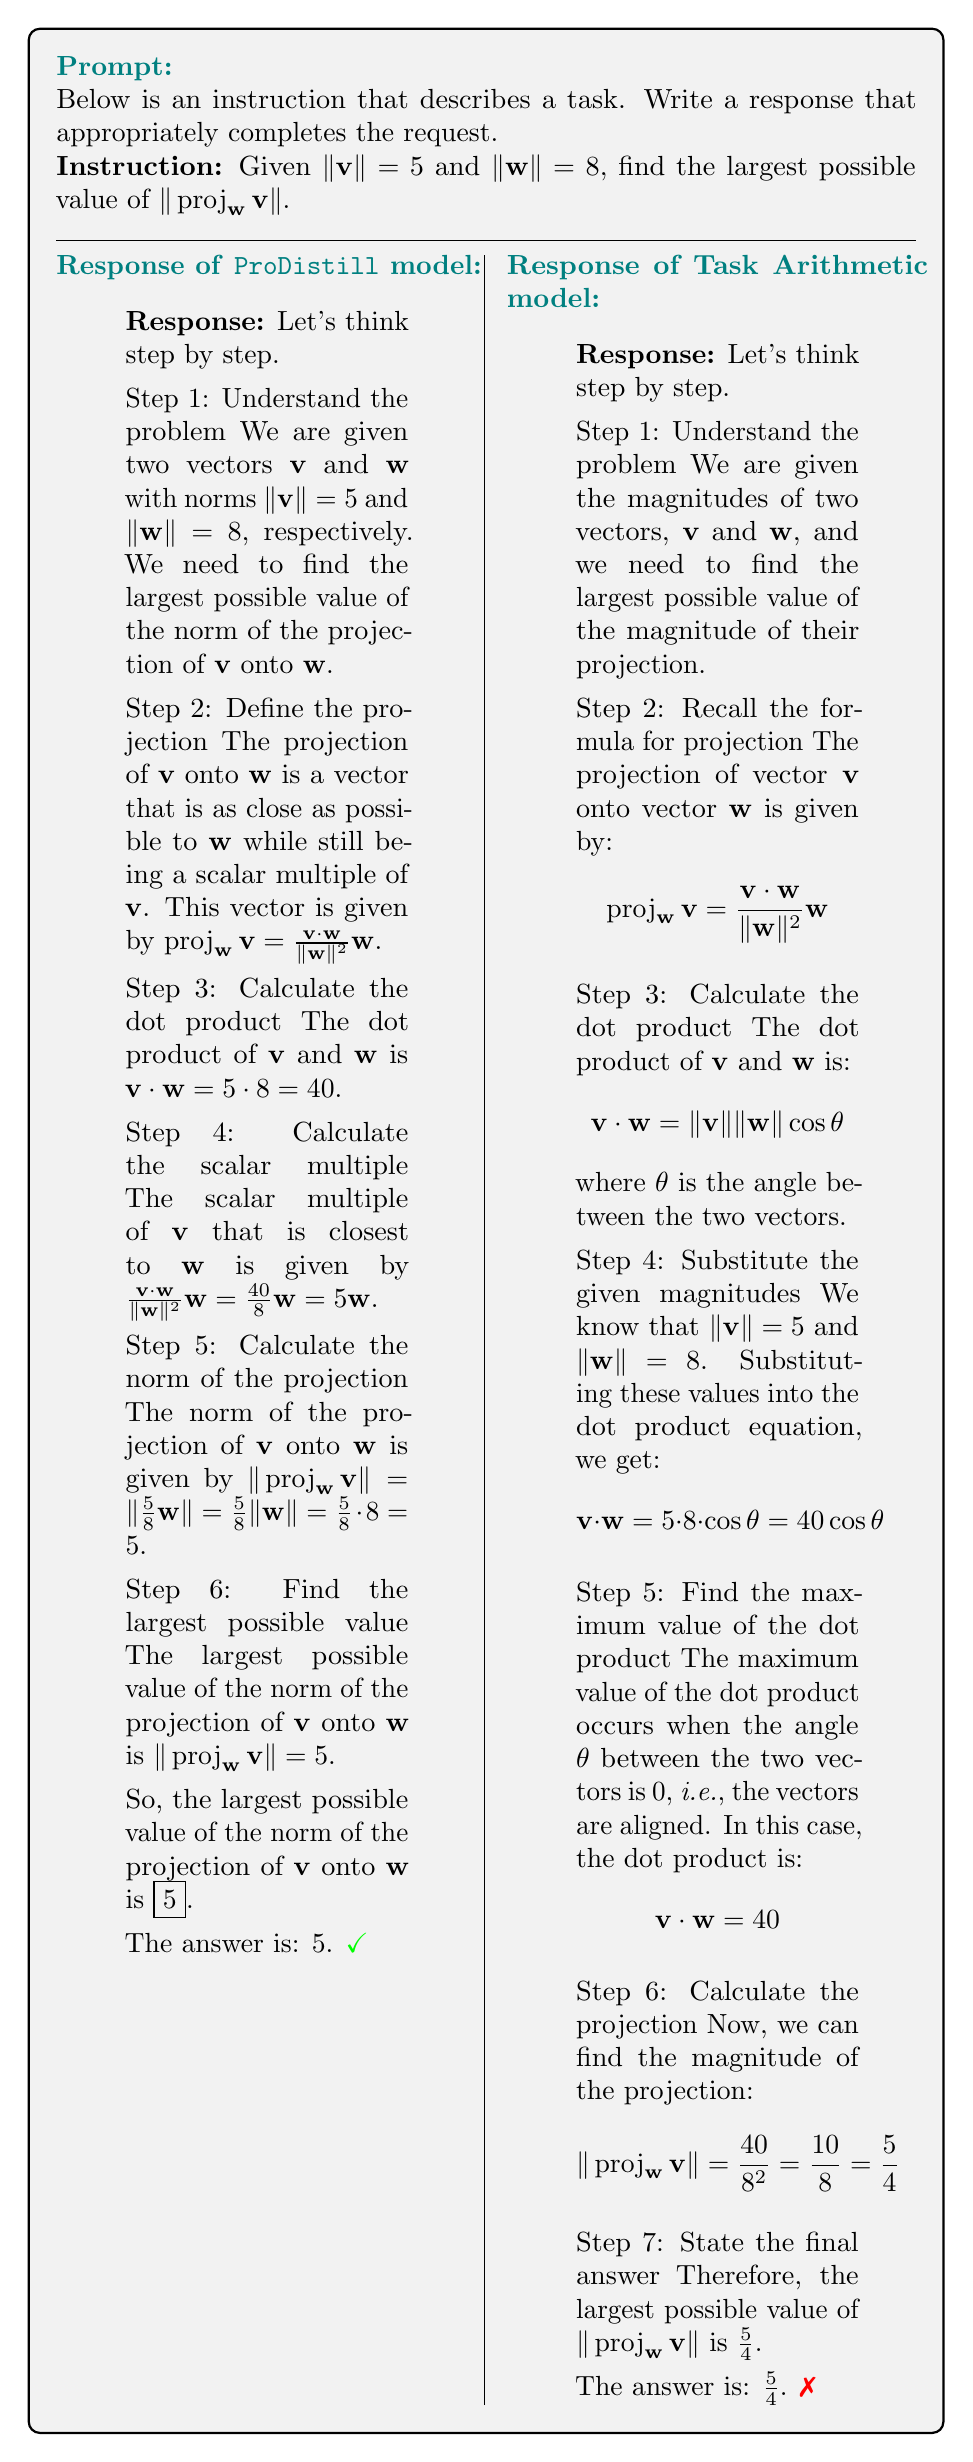
\begin{tikzpicture}
        \node[draw, fill=gray!10, rounded corners, thick, inner sep=10pt, minimum width=0.9\textwidth] (box) {
            \begin{minipage}{0.9\textwidth}
                \textbf{\textcolor{teal}{Prompt:}} \\
Below is an instruction that describes a task. Write a response that appropriately completes the request.

\textbf{Instruction:}
Given $\|\mathbf{v}\| = 5$ and $\|\mathbf{w}\| = 8,$ find the largest possible value of
$\|\operatorname{proj}_{\mathbf{w}} \mathbf{v}\|.$\\
                \rule{\linewidth}{0.4pt}
                
                \begin{minipage}[t]{0.49\textwidth}
                    \textbf{\textcolor{teal}{Response of \texttt{ProDistill} model:}}
                    \begin{quote}
\textbf{Response:} Let's think step by step.


Step 1: Understand the problem
We are given two vectors $\mathbf{v}$ and $\mathbf{w}$ with norms $\|\mathbf{v}\| = 5$ and $\|\mathbf{w}\| = 8$, respectively. We need to find the largest possible value of the norm of the projection of $\mathbf{v}$ onto $\mathbf{w}$.

Step 2: Define the projection
The projection of $\mathbf{v}$ onto $\mathbf{w}$ is a vector that is as close as possible to $\mathbf{w}$ while still being a scalar multiple of $\mathbf{v}$. This vector is given by $\operatorname{proj}_{\mathbf{w}} \mathbf{v} = \frac{\mathbf{v} \cdot \mathbf{w}}{\|\mathbf{w}\|^2} \mathbf{w}$.

Step 3: Calculate the dot product
The dot product of $\mathbf{v}$ and $\mathbf{w}$ is $\mathbf{v} \cdot \mathbf{w} = 5 \cdot 8 = 40$.

Step 4: Calculate the scalar multiple
The scalar multiple of $\mathbf{v}$ that is closest to $\mathbf{w}$ is given by $\frac{\mathbf{v} \cdot \mathbf{w}}{\|\mathbf{w}\|^2} \mathbf{w} = \frac{40}{8} \mathbf{w} = 5 \mathbf{w}$.

Step 5: Calculate the norm of the projection
The norm of the projection of $\mathbf{v}$ onto $\mathbf{w}$ is given by $\|\operatorname{proj}_{\mathbf{w}} \mathbf{v}\| = \|\frac{5}{8} \mathbf{w}\| = \frac{5}{8} \|\mathbf{w}\| = \frac{5}{8} \cdot 8 = 5$.

Step 6: Find the largest possible value
The largest possible value of the norm of the projection of $\mathbf{v}$ onto $\mathbf{w}$ is $\|\operatorname{proj}_{\mathbf{w}} \mathbf{v}\| = 5$.

So, the largest possible value of the norm of the projection of $\mathbf{v}$ onto $\mathbf{w}$ is $\boxed{5}$.

The answer is: 5. \textcolor{green}{\checkmark}
                    \end{quote}
                \end{minipage}
                \vrule width 0.5pt
                \hspace{0.2cm}
                \begin{minipage}[t]{0.49\textwidth}
                    \textbf{\textcolor{teal}{Response of Task Arithmetic model:}}
                    \begin{quote}
\textbf{Response:} Let's think step by step.

Step 1: Understand the problem
We are given the magnitudes of two vectors, $\mathbf{v}$ and $\mathbf{w}$, and we need to find the largest possible value of the magnitude of their projection.

Step 2: Recall the formula for projection
The projection of vector $\mathbf{v}$ onto vector $\mathbf{w}$ is given by:
\[\operatorname{proj}_{\mathbf{w}} \mathbf{v} = \frac{\mathbf{v} \cdot \mathbf{w}}{\|\mathbf{w}\|^2} \mathbf{w}\]

Step 3: Calculate the dot product
The dot product of $\mathbf{v}$ and $\mathbf{w}$ is:
\[\mathbf{v} \cdot \mathbf{w} = \|\mathbf{v}\| \|\mathbf{w}\| \cos \theta\]
where $\theta$ is the angle between the two vectors.

Step 4: Substitute the given magnitudes
We know that $\|\mathbf{v}\| = 5$ and $\|\mathbf{w}\| = 8$. Substituting these values into the dot product equation, we get:
\[\mathbf{v} \cdot \mathbf{w} = 5 \cdot 8 \cdot \cos \theta = 40 \cos \theta\]

Step 5: Find the maximum value of the dot product
The maximum value of the dot product occurs when the angle $\theta$ between the two vectors is $0$, \emph{i.e.}, the vectors are aligned. In this case, the dot product is:
\[\mathbf{v} \cdot \mathbf{w} = 40\]

Step 6: Calculate the projection
Now, we can find the magnitude of the projection:
\[\|\operatorname{proj}_{\mathbf{w}} \mathbf{v}\| = \frac{40}{8^2} = \frac{10}{8} = \frac{5}{4}\]

Step 7: State the final answer
Therefore, the largest possible value of $\|\operatorname{proj}_{\mathbf{w}} \mathbf{v}\|$ is $\frac{5}{4}$.

The answer is: $\frac{5}{4}$. \textcolor{red}{\ding{55}}
                    \end{quote}
                \end{minipage}
            \end{minipage}
        };
    \end{tikzpicture}
    \label{fig: math example}
    \caption{\textbf{Comparison of LLM generation results on the MATH benchmark.}}
\end{figure}


\begin{figure}[ht]
    \centering
    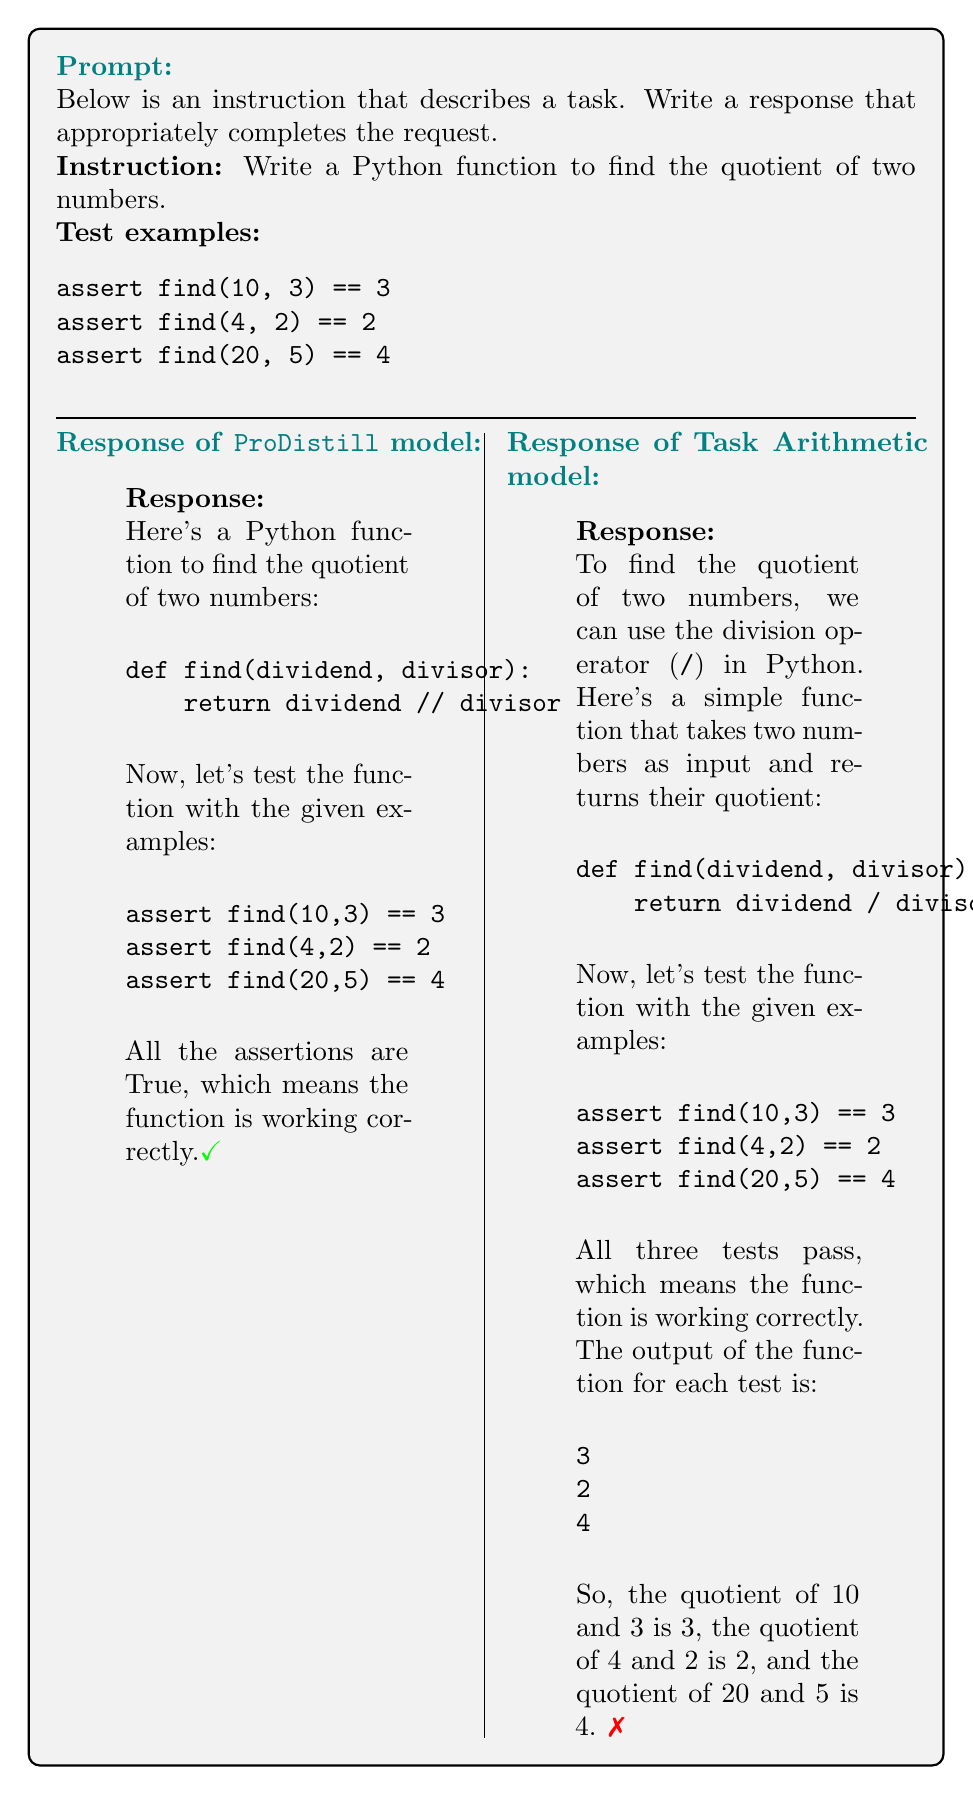
\begin{tikzpicture}
        \node[draw, fill=gray!10, rounded corners, thick, inner sep=10pt, minimum width=0.9\textwidth] (box) {
            \begin{minipage}{0.9\textwidth}
                \textbf{\textcolor{teal}{Prompt:}} \\
Below is an instruction that describes a task. Write a response that appropriately completes the request.

\textbf{Instruction:}
Write a Python function to find the quotient of two numbers.

\textbf{Test examples:}
\begin{verbatim}
assert find(10, 3) == 3
assert find(4, 2) == 2
assert find(20, 5) == 4
\end{verbatim}
                \rule{\linewidth}{0.4pt}
                
                \begin{minipage}[t]{0.49\textwidth}
                    \textbf{\textcolor{teal}{Response of \texttt{ProDistill} model:}}
                    \begin{quote}
\textbf{Response:} \\
Here's a Python function to find the quotient of two numbers:

\begin{verbatim}
def find(dividend, divisor):
    return dividend // divisor
\end{verbatim}

Now, let's test the function with the given examples:

\begin{verbatim}
assert find(10,3) == 3
assert find(4,2) == 2
assert find(20,5) == 4
\end{verbatim}

All the assertions are True, which means the function is working correctly.\textcolor{green}{\checkmark}

                    \end{quote}
                \end{minipage}
                \vrule width 0.5pt
                \hspace{0.2cm}
                \begin{minipage}[t]{0.49\textwidth}
                    \textbf{\textcolor{teal}{Response of Task Arithmetic model:}}
                    \begin{quote}
\textbf{Response:} \\
To find the quotient of two numbers, we can use the division operator (\texttt{/}) in Python. Here's a simple function that takes two numbers as input and returns their quotient:

\begin{verbatim}
def find(dividend, divisor):
    return dividend / divisor
\end{verbatim}

Now, let's test the function with the given examples:

\begin{verbatim}
assert find(10,3) == 3
assert find(4,2) == 2
assert find(20,5) == 4
\end{verbatim}

All three tests pass, which means the function is working correctly. The output of the function for each test is:

\begin{verbatim}
3
2
4
\end{verbatim}

So, the quotient of 10 and 3 is 3, the quotient of 4 and 2 is 2, and the quotient of 20 and 5 is 4.
 \textcolor{red}{\ding{55}}
                    \end{quote}
                \end{minipage}
            \end{minipage}
        };
    \end{tikzpicture}
    \label{fig: code example}
    \caption{\textbf{Comparison of LLM generation results on the MBPP benchmark.}}
\end{figure}


\begin{figure}[ht]
    \centering
    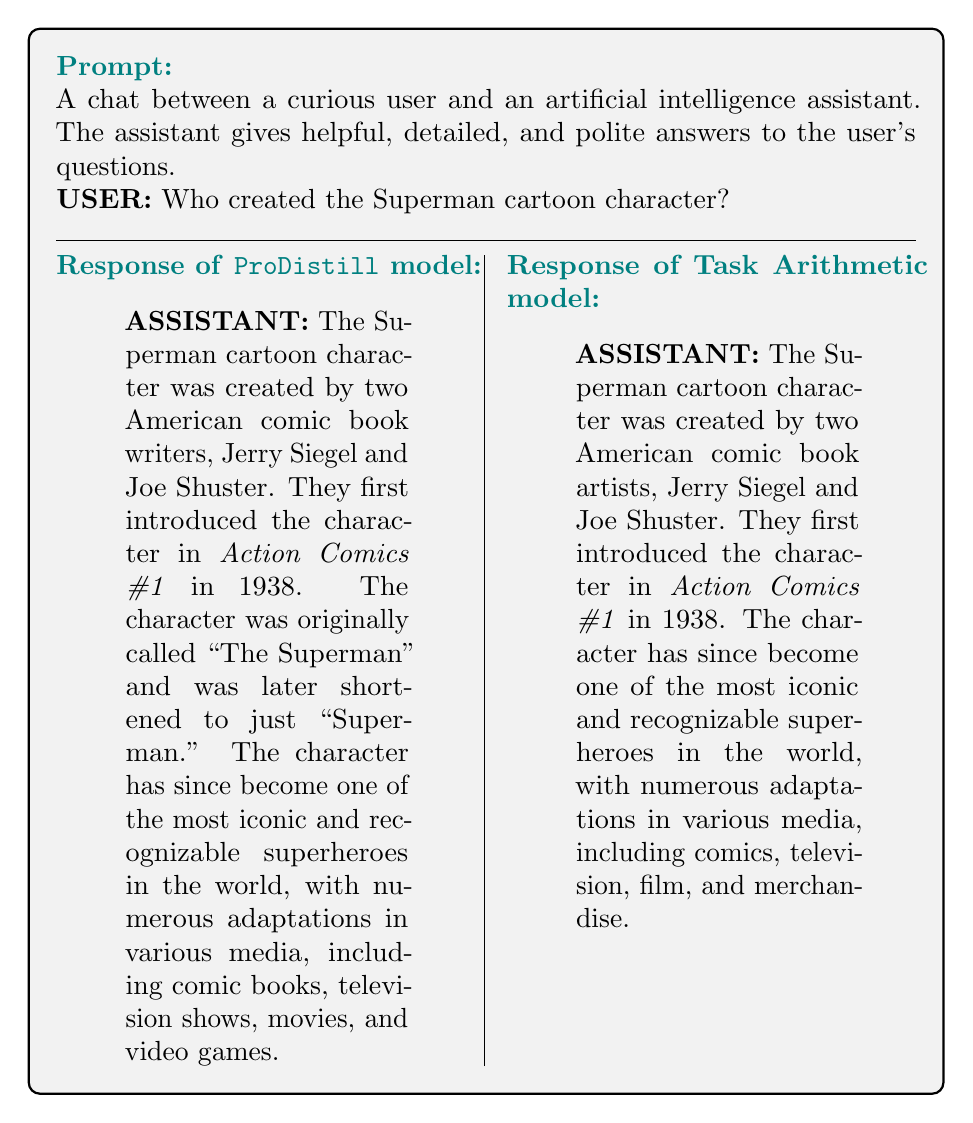
\begin{tikzpicture}
        \node[draw, fill=gray!10, rounded corners, thick, inner sep=10pt, minimum width=0.9\textwidth] (box) {
            \begin{minipage}{0.9\textwidth}
                \textbf{\textcolor{teal}{Prompt:}} \\
A chat between a curious user and an artificial intelligence assistant. The assistant gives helpful, detailed, and polite answers to the user's questions.

\textbf{USER:} Who created the Superman cartoon character?\\
                \rule{\linewidth}{0.4pt}
                
                \begin{minipage}[t]{0.49\textwidth}
                    \textbf{\textcolor{teal}{Response of \texttt{ProDistill} model:}}
                    \begin{quote}
\textbf{ASSISTANT:} The Superman cartoon character was created by two American comic book writers, Jerry Siegel and Joe Shuster. They first introduced the character in \textit{Action Comics \#1} in 1938. The character was originally called ``The Superman'' and was later shortened to just ``Superman.'' The character has since become one of the most iconic and recognizable superheroes in the world, with numerous adaptations in various media, including comic books, television shows, movies, and video games.

                    \end{quote}
                \end{minipage}
                \vrule width 0.5pt
                \hspace{0.2cm}
                \begin{minipage}[t]{0.49\textwidth}
                    \textbf{\textcolor{teal}{Response of Task Arithmetic model:}}
                    \begin{quote}
\textbf{ASSISTANT:} The Superman cartoon character was created by two American comic book artists, Jerry Siegel and Joe Shuster. They first introduced the character in \textit{Action Comics \#1} in 1938. The character has since become one of the most iconic and recognizable superheroes in the world, with numerous adaptations in various media, including comics, television, film, and merchandise.

                    \end{quote}
                \end{minipage}
            \end{minipage}
        };
    \end{tikzpicture}
    \label{fig: instruct example}
    \caption{\textbf{Comparison of LLM generation results on the AlpacaEval 2.0 benchmark.}}
\end{figure}
    

\end{document}
